\documentclass[12pt,oneside]{book}

%%%%%%%%%%%%%%%%%%%%%%%%%%%%%%%%%%%%%%%%%%%%%%%%%%%%%%%%%%%%%%%%%%%%%%%%%%%%%%%%%%%%%%%%%%%%%%%%%%%
%                                                                                                 %
% The mathematical style of these documents follows                                               %
%                                                                                                 %
% A. Thompson and B.N. Taylor. The NIST Guide for the Use of the International System of Units.   %
%    NIST Special Publication 881, 2008.                                                          %
%                                                                                                 %
% http://www.nist.gov/pml/pubs/sp811/index.cfm                                                    %
%                                                                                                 %
%%%%%%%%%%%%%%%%%%%%%%%%%%%%%%%%%%%%%%%%%%%%%%%%%%%%%%%%%%%%%%%%%%%%%%%%%%%%%%%%%%%%%%%%%%%%%%%%%%%

% $Date: 2013-11-26 10:43:59 -0500 (Tue, 26 Nov 2013) $
% $Revision: 17538 $
% $Author: gforney $

%%%%%%%%%%%%%%%%%%%%%%%%%%%%%%%%%%%%%%%%%%%%%%%%%%%%%%%%%%%%%%%%%%%%%%%%%%%%%%%%%%%%%%%%%%%%%%%%%%%
%                                                                                                 %
% The mathematical style of these documents follows                                               %
%                                                                                                 %
% A. Thompson and B.N. Taylor. The NIST Guide for the Use of the International System of Units.   %
%    NIST Special Publication 881, 2008.                                                          %
%                                                                                                 %
% http://www.nist.gov/pml/pubs/sp811/index.cfm                                                    %
%                                                                                                 %
%%%%%%%%%%%%%%%%%%%%%%%%%%%%%%%%%%%%%%%%%%%%%%%%%%%%%%%%%%%%%%%%%%%%%%%%%%%%%%%%%%%%%%%%%%%%%%%%%%%

% Packages which force the use of better TeX coding
% Mostly from http://tex.stackexchange.com/q/19264
%%\RequirePackage[l2tabu, orthodox]{nag}
%%\usepackage{fixltx2e}
%\usepackage{isomath} % Disabled for the moment because it changes the syntax for bold and roman Greek math symbols
%%\usepackage[all,warning]{onlyamsmath}
%\usepackage{strict} % Commented out for now because it is uncommon. A copy of style.sty is in Manuals/LaTeX_Style_Files/.

\usepackage{times,mathptmx}
\usepackage[pdftex]{graphicx}
\usepackage{tabularx,ragged2e,booktabs,caption}
\usepackage{multirow}
\usepackage{pdfsync}
\usepackage{tikz}
\usepackage{pgfplots}
%\pgfplotsset{compat=1.7}
\usepackage{tocloft}
\usepackage{color}
\usepackage{amsmath}
\definecolor{linknavy}{rgb}{0,0,0.50196}
\definecolor{linkred}{rgb}{1,0,0}
\definecolor{linkblue}{rgb}{0,0,1}
\usepackage{float}
\usepackage{caption}
\usepackage{graphpap}
\usepackage{rotating}
\usepackage{graphicx}
\usepackage{geometry}
\usepackage{relsize}
\usepackage{longtable}
\usepackage{lscape}
\usepackage{amssymb}
\usepackage{makeidx} % Create index at end of document
\usepackage[nottoc,notlof,notlot]{tocbibind} % Put the bibliography and index in the ToC
\usepackage{lastpage} % Automatic last page number reference.
\usepackage[T1]{fontenc}
\usepackage{enumerate}
\usepackage{upquote}
\usepackage{moreverb}
\usepackage{xfrac}
\usepackage{cite}

\newcommand{\nopart}{\expandafter\def\csname Parent-1\endcsname{}} % To fix table of contents in pdf.
\newcommand{\ct}{\tt\small} % eventually will be deprecated due to http://www.tex.ac.uk/cgi-bin/texfaq2html?label=2letterfontcmd
\newcommand{\textct}[1]{\texttt{\small #1}}

\usepackage{tocstyle} % Fix table of contents sections from overlapping section titles
\usetocstyle{standard}
\usepackage{siunitx}
\sisetup{
    detect-all = true,
    input-decimal-markers = {.},
    input-ignore = {,},
    inter-unit-product = \ensuremath{{}\cdot{}},
    multi-part-units = repeat,
    number-unit-product = \text{~},
    per-mode = fraction,
    separate-uncertainty = true,
}

\usepackage{listings}
\usepackage{textcomp}
\definecolor{lbcolor}{rgb}{0.96,0.96,0.96}
\lstset{
    %backgroundcolor=\color{lbcolor},
    tabsize=4,
    rulecolor=,
    language=Fortran,
        basicstyle=\footnotesize\ttfamily,
        upquote=true,
        aboveskip={\baselineskip},
        belowskip={\baselineskip},
        columns=fixed,
        extendedchars=true,
        breaklines=true,
        breakatwhitespace=true,
        frame=none,
        showtabs=false,
        showspaces=false,
        showstringspaces=false,
        identifierstyle=\ttfamily,
        keywordstyle=\color[rgb]{0,0,0},
        commentstyle=\color[rgb]{0,0,0},
        stringstyle=\color[rgb]{0,0,0},
}

\usepackage[pdftex,
        colorlinks=true,
        urlcolor=linkblue,     % \href{...}{...} external (URL)
        citecolor=linkred,     % citation number colors
        linkcolor=linknavy,    % \ref{...} and \pageref{...}
        pdfproducer={pdflatex},
        pdfpagemode=UseNone,
        bookmarksopen=true,
        plainpages=false,
        verbose]{hyperref}

% The Following commented code makes the ``Draft'' watermark on each page.
%\usepackage{eso-pic}
%\usepackage{type1cm}
%\makeatletter
%   \AddToShipoutPicture{
%     \setlength{\@tempdimb}{.5\paperwidth}
%     \setlength{\@tempdimc}{.5\paperheight}
%     \setlength{\unitlength}{1pt}
%     \put(\strip@pt\@tempdimb,\strip@pt\@tempdimc){
%     \makebox(0,0){\rotatebox{45}{\textcolor[gray]{0.75}{\fontsize{8cm}\selectfont{RC6}}}}}
% }
%\makeatother

\setlength{\textwidth}{6.5in}
\setlength{\textheight}{9.0in}
\setlength{\topmargin}{0.in}
\setlength{\headheight}{0.pt}
\setlength{\headsep}{0.in}
\setlength{\parindent}{0.25in}
\setlength{\oddsidemargin}{0.0in}
\setlength{\evensidemargin}{0.0in}
\setlength{\leftmargini}{\parindent} % Controls the indenting of the "bullets" in a list
\setlength{\cftsecnumwidth}{0.45in}
\setlength{\cftsubsecnumwidth}{0.5in}
\setlength{\cftfignumwidth}{0.45in}
\setlength{\cfttabnumwidth}{0.45in}

\newcommand{\titlesigs}
{
\small
\flushright{U.S. Department of Commerce \\
{\em Penny Pritzker, Secretary} \\
\hspace{1in} \\
National Institute of Standards and Technology \\
{\em Willie May, Under Secretary of Commerce for Standards and Technology and Acting Director} }
}

% commands to use for "official" cover and title pages
% see smokeview verification guide to see how they are used

\newcommand{\headerA}[1]{
\flushright{
\fontsize{20}{24}\selectfont
\bf{NIST Special Publication #1}}
}

\newcommand{\headerB}[1]{
\flushright{
\fontsize{28}{33.6}\selectfont
\bf{#1}
}
}

\newcommand{\headerC}[1]{
\vspace{.5in}
\flushright{\fontsize{14}{16.8}\selectfont
#1}
}

\frenchspacing

\newcommand{\dod}[2]{\frac{\partial #1}{\partial #2}}
\newcommand{\DoD}[2]{\frac{\mathrm{D} #1}{\mathrm{D} #2}}
\newcommand{\dsods}[2]{\frac{\partial^2 #1}{\partial #2^2}}
\renewcommand{\d}{\,\mathrm{d}}
\newcommand{\dx}{\delta x}
\newcommand{\dy}{\delta y}
\newcommand{\dz}{\delta z}
\newcommand{\degF}{$^\circ$F}
\newcommand{\degC}{$^\circ$C}
\newcommand{\x}{x}
\newcommand{\y}{y}
\newcommand{\z}{z}
\newcommand{\dt}{\delta t}
\newcommand{\dn}{\delta n}
\newcommand{\cH}{H}
\newcommand{\hu}{u}
\newcommand{\hv}{v}
\newcommand{\hw}{w}
\newcommand{\la}{\lambda}
\newcommand{\bO}{{\Omega}}
\newcommand{\bo}{{\mathbf{\omega}}}
\newcommand{\btau}{\mathbf{\tau}}
\newcommand{\bdelta}{{\mathbf{\delta}}}
\newcommand{\sumyw}{\sum (Y_\alpha/W_\alpha)}
\newcommand{\oW}{\overline{W}}
\newcommand{\om}{\ensuremath{\omega}}
\newcommand{\omx}{\omega_x}
\newcommand{\omy}{\omega_y}
\newcommand{\omz}{\omega_z}
\newcommand{\erf}{\hbox{erf}}
\newcommand{\erfc}{\hbox{erfc}}
\newcommand{\bF}{{\mathbf{F}}}
\newcommand{\bG}{{\mathbf{G}}}
\newcommand{\bof}{{\mathbf{f}}}
\newcommand{\bq}{{\mathbf{q}}}
\newcommand{\br}{{\mathbf{r}}}
\newcommand{\bu}{{\mathbf{u}}}
\newcommand{\bx}{{\mathbf{x}}}
\newcommand{\bk}{{\mathbf{k}}}
\newcommand{\bv}{{\mathbf{v}}}
\newcommand{\bg}{{\mathbf{g}}}
\newcommand{\bn}{{\mathbf{n}}}
\newcommand{\bS}{{\mathbf{S}}}
\newcommand{\bW}{\overline{W}}
\newcommand{\dS}{d{\mathbf{S}}}
\newcommand{\bs}{{\mathbf{s}}}
\newcommand{\bI}{{\mathbf{I}}}
\newcommand{\hp}{H}
\newcommand{\trho}{\tilde{\rho}}
\newcommand{\dph}{{\delta\phi}}
\newcommand{\dth}{{\delta\theta}}
\newcommand{\tp}{\tilde{p}}
\newcommand{\bp}{\overline{p}}
\newcommand{\dQ}{\dot{Q}}
\newcommand{\dq}{\dot{q}}
\newcommand{\dbq}{\dot{\mathbf{q}}}
\newcommand{\dm}{\dot{m}}
\newcommand{\ha}{\frac{1}{2}}
\newcommand{\ft}{\frac{4}{3}}
\newcommand{\ot}{\frac{1}{3}}
\newcommand{\fofi}{\frac{4}{5}}
\newcommand{\of}{\frac{1}{4}}
\newcommand{\twth}{\frac{2}{3}}
\newcommand{\R}{R}
\newcommand{\be}{\begin{equation}}
\newcommand{\ee}{\end{equation}}
\newcommand{\RE}{\hbox{Re}}
\newcommand{\LE}{\hbox{Le}}
\newcommand{\PR}{\hbox{Pr}}
\newcommand{\PE}{\hbox{Pe}}
\newcommand{\NU}{\hbox{Nu}}
\newcommand{\SC}{\hbox{Sc}}
\newcommand{\SH}{\hbox{Sh}}
\newcommand{\WE}{\hbox{We}}
\newcommand{\COTWO}{\text{\tiny \hbox{CO}$_2$}}
\newcommand{\HTWOO}{\text{\tiny \hbox{H}$_2$\hbox{O}}}
\newcommand{\OTWO}{\text{\tiny \hbox{O}$_2$}}
\newcommand{\NTWO}{\text{\tiny \hbox{N}$_2$}}
\newcommand{\CO}{\text{\tiny \hbox{CO}}}
\newcommand{\F}{\text{\tiny \hbox{F}}}
\newcommand{\C}{\text{\tiny \hbox{C}}}
\newcommand{\Hy}{\text{\tiny \hbox{H}}}
\newcommand{\So}{\text{\tiny \hbox{S}}}
\newcommand{\M}{\text{\tiny \hbox{M}}}
\newcommand{\xx}{\text{\tiny \hbox{x}}}
\newcommand{\yy}{\text{\tiny \hbox{y}}}
\newcommand{\zz}{\text{\tiny \hbox{z}}}
\newcommand{\smvlines}{115~000}

\newcommand{\calH}{\mathcal{H}}
\newcommand{\calR}{\mathcal{R}}

\newcommand{\dif}{\mathrm{d}}
\newcommand{\Div}{\nabla\cdot}
\newcommand{\D}{\mbox{D}}
\newcommand{\mhalf}{\mbox{$\frac{1}{2}$}}
\newcommand{\thalf}{\mbox{\tiny $\frac{1}{2}$}}
\newcommand{\tripleprime}{{\prime\prime\prime}}
\newcommand{\ppp}{{\prime\prime\prime}}
\newcommand{\pp}{{\prime\prime}}

\newcommand{\superscript}[1]{\ensuremath{^{\textrm{\tiny #1}}}}
\newcommand{\subscript}[1]{\ensuremath{_{\textrm{\tiny #1}}}}

\newcommand{\rb}[1]{\raisebox{1.5ex}[0pt]{#1}}

\newcommand{\Ra}{$\Rightarrow$}
\newcommand{\hhref}[1]{\href{#1}{{\tt #1}}}
\newcommand{\fdsinput}[1]{{\scriptsize\verbatiminput{../../Verification/Visualization/#1}}}

\definecolor{AQUAMARINE}{rgb}{0.49804,1.00000,0.83137}
\definecolor{ANTIQUE WHITE}{rgb}{0.98039,0.92157,0.84314}
\definecolor{BEIGE}{rgb}{0.96078,0.96078,0.86275}
\definecolor{BLACK}{rgb}{0.00000,0.00000,0.00000}
\definecolor{BLUE}{rgb}{0.00000,0.00000,1.00000}
\definecolor{BLUE VIOLET}{rgb}{0.54118,0.16863,0.88627}
\definecolor{BRICK}{rgb}{0.61176,0.40000,0.12157}
\definecolor{BROWN}{rgb}{0.64706,0.16471,0.16471}
\definecolor{BURNT SIENNA}{rgb}{0.54118,0.21176,0.05882}
\definecolor{BURNT UMBER}{rgb}{0.54118,0.20000,0.14118}
\definecolor{CADET BLUE}{rgb}{0.37255,0.61961,0.62745}
\definecolor{CHOCOLATE}{rgb}{0.82353,0.41176,0.11765}
\definecolor{COBALT}{rgb}{0.23922,0.34902,0.67059}
\definecolor{CORAL}{rgb}{1.00000,0.49804,0.31373}
\definecolor{CYAN}{rgb}{0.00000,1.00000,1.00000}
\definecolor{DIMGRAY }{rgb}{0.41176,0.41176,0.41176}
\definecolor{EMERALD GREEN}{rgb}{0.00000,0.78824,0.34118}
\definecolor{FIREBRICK}{rgb}{0.69804,0.13333,0.13333}
\definecolor{FLESH}{rgb}{1.00000,0.49020,0.25098}
\definecolor{FOREST GREEN}{rgb}{0.13333,0.54510,0.13333}
\definecolor{GOLD }{rgb}{1.00000,0.84314,0.00000}
\definecolor{GOLDENROD}{rgb}{0.85490,0.64706,0.12549}
\definecolor{GRAY}{rgb}{0.50196,0.50196,0.50196}
\definecolor{GREEN}{rgb}{0.00000,1.00000,0.00000}
\definecolor{GREEN YELLOW}{rgb}{0.67843,1.00000,0.18431}
\definecolor{HONEYDEW}{rgb}{0.94118,1.00000,0.94118}
\definecolor{HOT PINK}{rgb}{1.00000,0.41176,0.70588}
\definecolor{INDIAN RED}{rgb}{0.80392,0.36078,0.36078}
\definecolor{INDIGO}{rgb}{0.29412,0.00000,0.50980}
\definecolor{IVORY}{rgb}{1.00000,1.00000,0.94118}
\definecolor{IVORY BLACK}{rgb}{0.16078,0.14118,0.12941}
\definecolor{KELLY GREEN}{rgb}{0.00000,0.50196,0.00000}
\definecolor{KHAKI}{rgb}{0.94118,0.90196,0.54902}
\definecolor{LAVENDER}{rgb}{0.90196,0.90196,0.98039}
\definecolor{LIME GREEN}{rgb}{0.19608,0.80392,0.19608}
\definecolor{MAGENTA}{rgb}{1.00000,0.00000,1.00000}
\definecolor{MAROON}{rgb}{0.50196,0.00000,0.00000}
\definecolor{MELON}{rgb}{0.89020,0.65882,0.41176}
\definecolor{MIDNIGHT BLUE}{rgb}{0.09804,0.09804,0.43922}
\definecolor{MINT}{rgb}{0.74118,0.98824,0.78824}
\definecolor{NAVY}{rgb}{0.00000,0.00000,0.50196}
\definecolor{OLIVE}{rgb}{0.50196,0.50196,0.00000}
\definecolor{OLIVE DRAB}{rgb}{0.41961,0.55686,0.13725}
\definecolor{ORANGE}{rgb}{1.00000,0.50196,0.00000}
\definecolor{ORANGE RED}{rgb}{1.00000,0.27059,0.00000}
\definecolor{ORCHID}{rgb}{0.85490,0.43922,0.83922}
\definecolor{PINK}{rgb}{1.00000,0.75294,0.79608}
\definecolor{POWDER BLUE}{rgb}{0.69020,0.87843,0.90196}
\definecolor{PURPLE}{rgb}{0.50196,0.00000,0.50196}
\definecolor{RASPBERRY}{rgb}{0.52941,0.14902,0.34118}
\definecolor{RED}{rgb}{1.00000,0.00000,0.00000}
\definecolor{ROYAL BLUE}{rgb}{0.25490,0.41176,0.88235}
\definecolor{SALMON}{rgb}{0.98039,0.50196,0.44706}
\definecolor{SANDY BROWN}{rgb}{0.95686,0.64314,0.37647}
\definecolor{SEA GREEN}{rgb}{0.32941,1.00000,0.62353}
\definecolor{SEPIA}{rgb}{0.36863,0.14902,0.07059}
\definecolor{SIENNA}{rgb}{0.62745,0.32157,0.17647}
\definecolor{SILVER}{rgb}{0.75294,0.75294,0.75294}
\definecolor{SKY BLUE}{rgb}{0.52941,0.80784,0.92157}
\definecolor{SLATEBLUE}{rgb}{0.41569,0.35294,0.80392}
\definecolor{SLATE GRAY}{rgb}{0.43922,0.50196,0.56471}
\definecolor{SPRING GREEN}{rgb}{0.00000,1.00000,0.49804}
\definecolor{STEEL BLUE}{rgb}{0.27451,0.50980,0.70588}
\definecolor{TAN}{rgb}{0.82353,0.70588,0.54902}
\definecolor{TEAL}{rgb}{0.00000,0.50196,0.50196}
\definecolor{THISTLE}{rgb}{0.84706,0.74902,0.84706}
\definecolor{TOMATO }{rgb}{1.00000,0.38824,0.27843}
\definecolor{TURQUOISE}{rgb}{0.25098,0.87843,0.81569}
\definecolor{VIOLET}{rgb}{0.93333,0.50980,0.93333}
\definecolor{VIOLET RED}{rgb}{0.81569,0.12549,0.56471}
\definecolor{WHITE}{rgb}{1.00000,1.00000,1.00000}
\definecolor{YELLOW}{rgb}{1.00000,1.00000,0.00000}

\pgfplotsset{
	colormap={blackwhite}{[5pt]
		rgb255(0pt)=(0,0,255); 
		rgb255(100pt)=(0,255,255); 
		rgb255(200pt)=(0,255,0); 
		rgb255(300pt)=(255,255,0); 
		rgb255(400pt)=(255,0,0)
	},
} % defines smokeview colorbar


\floatstyle{boxed}
\newfloat{notebox}{H}{lon}
\newfloat{warning}{H}{low}

% Set default longtable alignment
\setlength\LTleft{0pt}
\setlength\LTright{0pt}


% Rename chapter headings
\renewcommand{\chaptername}{Section}
\renewcommand{\bibname}{References}

% Math shortcuts
\renewcommand{\sb}[1]{_\mathrm{#1}}
\renewcommand{\C}{\mbox{C}}
\renewcommand{\H}{\mbox{H}}
\renewcommand{\O}{\mbox{O}}
\newcommand{\N}{\mbox{N}}
\newcommand{\Cl}{\mbox{Cl}}
\newcommand{\HCl}{\mbox{HCl}}

\usepackage{fancyhdr}
\pagestyle{fancy}
\lhead{}
\rhead{}
\chead{}
\renewcommand{\headrulewidth}{0pt}

\hypersetup{
  pdftitle={Design Fires for Emission Control System Commissioning},
  pdfauthor={Weinschenk, Craig G and Bundy, Matthew}, 
  pdfsubject={} 
  } 

\begin{document}
\pagenumbering{gobble}

\bibliographystyle{unsrt}
%\pagestyle{empty}

\begin{minipage}[t][9in][s]{6.25in}

\begin{flushright}
\fontsize{20}{24}\selectfont
\bf{NIST Technical Note XXXX}
\end{flushright}

\headerB{
Design Fires for Emission \\
Control System Commissioning\\
}

\normalsize

\headerC{
{
\flushright{
Craig G. Weinschenk \\
Matt Bundy \\

\vspace*{2\baselineskip}

\begingroup
\hypersetup{urlcolor=black}
\href{http://dx.doi.org/10.6028/NIST.TN.1838}{http://dx.doi.org/10.6028/NIST.TN.XXXX}
\endgroup
}

\vfill

\flushright{


\includegraphics[width=2.in]{../../../Bibliography/nistident_flright_vec} \\[.3in]
}
}
}

\end{minipage}

\newpage
\hspace{5in}
\newpage

\frontmatter

\begin{minipage}[t][9in][s]{6.25in}
\pagenumbering{gobble}

\begin{flushright}
\fontsize{20}{24}\selectfont
\bf{NIST Technical Note XXXX}
\end{flushright}

\headerB{
Design Fires for Emission \\
Control System Commissioning\\
}

\headerC{
\flushright{
Craig G. Weinschenk \\
Matthew Bundy \\
{\em Fire Research Division \\
Engineering Laboratory} \\

\vspace*{2\baselineskip}

\begingroup
\hypersetup{urlcolor=black}
\href{http://dx.doi.org/10.6028/NIST.TN.1838}{http://dx.doi.org/10.6028/NIST.TN.XXXX} \\
\endgroup

\vspace*{2\baselineskip}

August 2014}}

\vfill

\flushright{
\includegraphics[width=1in]{../../../Bibliography/doc} }

\titlesigs

\end{minipage}

\newpage

\begin{minipage}[t][9in][s]{6.25in}
\pagenumbering{gobble}

\flushright{Certain commercial entities, equipment, or materials may be identified in this \\
document in order to describe an experimental procedure or concept adequately. \\
Such identification is not intended to imply recommendation or endorsement by the \\
National Institute of Standards and Technology, nor is it intended to imply that the \\
entities, materials, or equipment are necessarily the best available for the purpose. \\
}

\vspace{3in}

\large
\flushright{\bf National Institute of Standards and Technology Technical Note XXXX \\
Natl.~Inst.~Stand.~Technol.~Tech.~Note~XXXX, \pageref{LastPage} pages (August 2014) \\
% http://dx.doi.org/10.6028/NIST.TN.XXXX \\
CODEN: NTNOEF }

\vfill

\hspace{1in}

\end{minipage}

\newpage

\frontmatter

\pagestyle{plain}
\pagenumbering{roman}
\setcounter{page}{3}

\cleardoublepage
\phantomsection
\addcontentsline{toc}{chapter}{Contents}
\tableofcontents

\cleardoublepage
\phantomsection
\addcontentsline{toc}{chapter}{List of Figures}
\listoffigures

\cleardoublepage
\phantomsection
\addcontentsline{toc}{chapter}{List of Tables}
\listoftables

\chapter{List of Acronyms}

\begin{tabbing}
\hspace{1.5in} \= \\
FDS \> Fire Dynamics Simulator \\
HRR \> Heat Release Rate \\
NIST \> National Institute of Standards and Technology \\
\end{tabbing}

\mainmatter

\chapter*{\centering Abstract}
\addcontentsline{toc}{chapter}{Abstract}
\pagenumbering{gobble}

\chapter{Introduction}
\pagenumbering{arabic}
\setcounter{page}{1}
The National Fire Research Laboratory (NFRL) is a fire test facility operated by the Engineering Laboratory at the National Institute of Standards and Technology (NIST). The NFRL is undergoing an expansion in order to provide additional research capabilities: test the performance of full-scale structures subjected to realistic fires and structural loading under controlled laboratory conditions, develop an experimental database on the performance of large-scale structural connections, components, sub-assemblies, and systems under realistic fire and loading, validate physics-based models to predict fire resistance performance of structures and enable performance-based standards for fire resistance design of structures and foster innovations in design and construction. To complete construction on the NFRL expansion, the updated emission control system needs to be tested to ensure the design specifications are achieved. This document will describe the source fires, appropriate lab safety, and test procedures. The objective of the fire tests is to use specifically designed source fires to test the emission control systems of the newly constructed fire research facility addition. The experiments are designed to ensure the system can handle elevated temperatures (gas burner), toxic gases (wood cribs with PVC), and particulates (group A commodities).

\chapter{Test Fires}
\label{test_fire}
The commissioning fires will take place in the pre-expansion laboratory space under a 9 m by 12 m oxygen-consumption calorimetry hood. The fuel packages will be centered under the hood, which is 6.4 m above the test floor. A flexible curtain, in place to contain combustion products, hangs 1.5 m below the lower edge of hood. Fig.~(\ref{fig:NFRL_fire}) shows a 2 MW natural gas fire under the hood during an experiment prior to the lab expansion. Note, that in the current configuration the wall to the left of the burner has been replaced by a roll-up door. The roll-up door provides access to the new testing space.

\begin{figure}
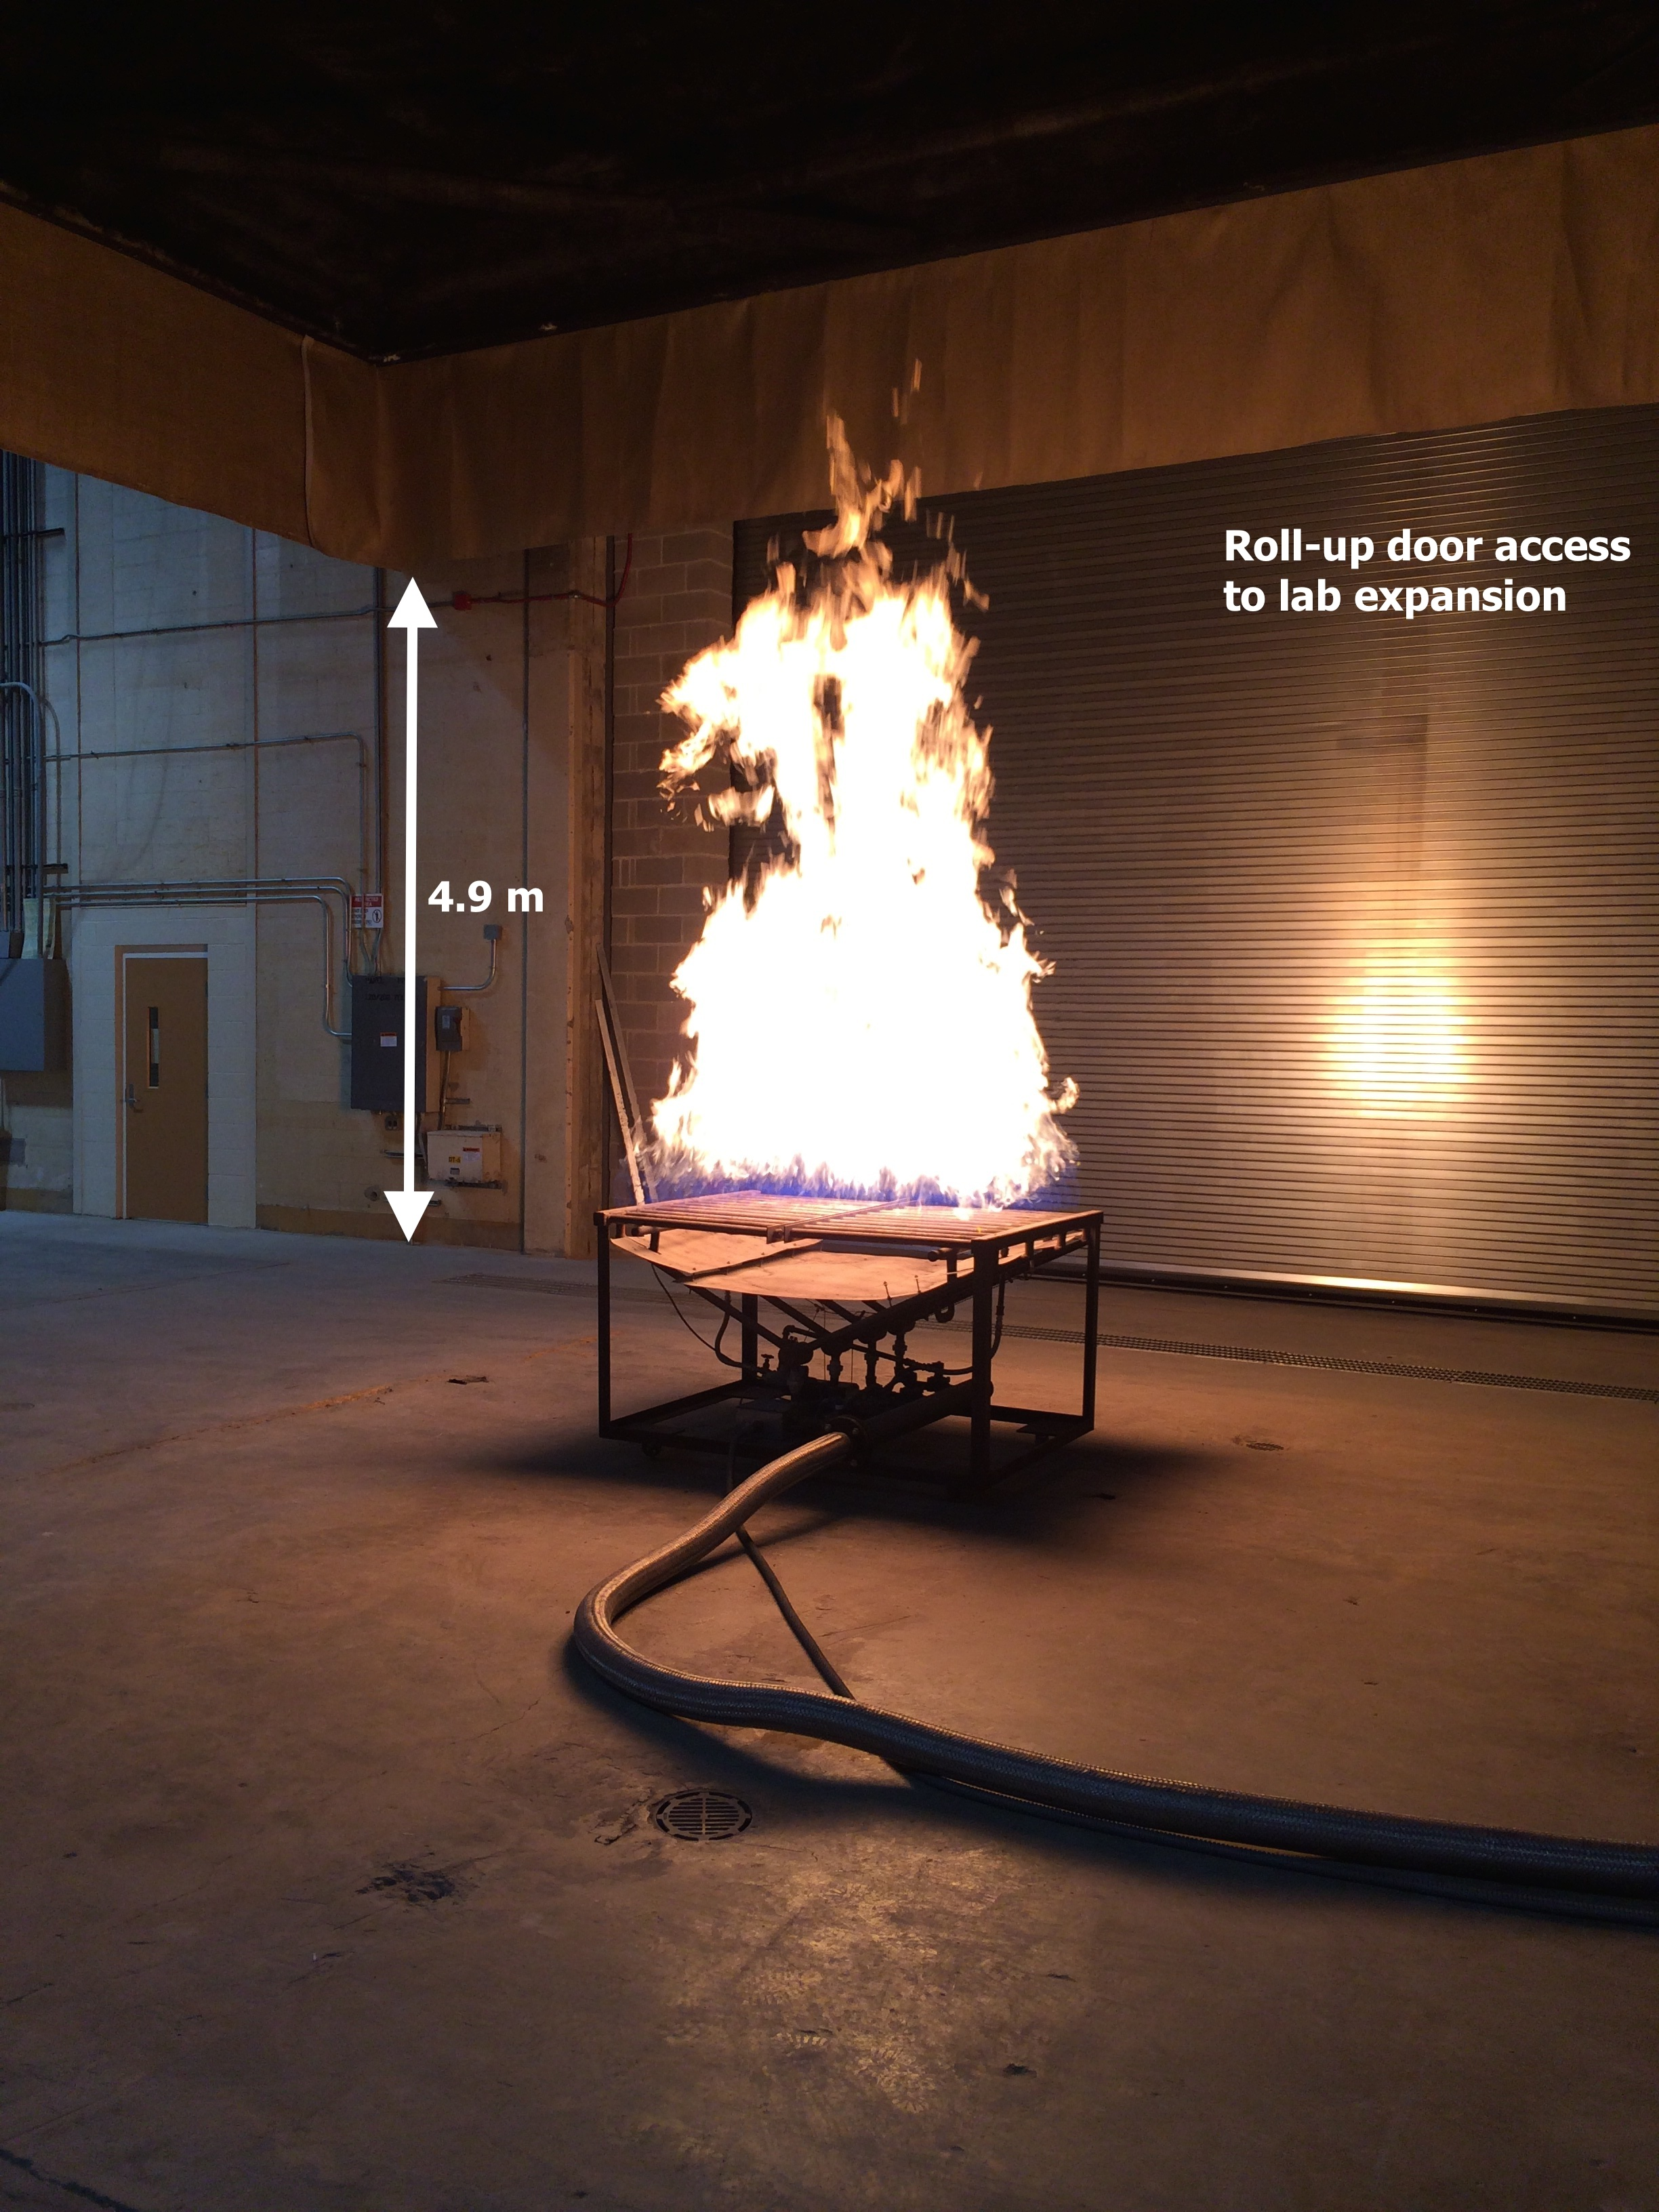
\includegraphics[width=\textwidth]{../Figures/NFRL_Fire}
\caption {Natural gas test burn in pre-construction NFRL.}
\label{fig:NFRL_fire}
\end{figure}

Based on the general experimental configuration shown in Fig.~(\ref{fig:NFRL_fire}) and \ref{app:nfrl_images}, Table ~\ref{tab:fires} outlines the fire tests to be conducted. The duplicity of tests is that similar to the existing system, the new ECS features two trains. Therefore, the scrubbing system in each train needs to be tested independently. 

\begin{table}
\centering
\caption{Design fires for ECS commissioning tests}
\label{tab:fires}
\begin{tabular}{ccccc}
\toprule[1.5pt]
Test ID & Fuel & Peak HRR (MW) & Burn Time (min) & Test Goal  \\
\midrule
1-3  & Natural Gas  & 2-8   & 60  & Temperature  \\
4  & Wood w/ PVC  & $\approx$ 1.5-2 & $\approx$ 50  & Acid, Train 3 \\
5  & Group A Comm. & $\approx$ 3 & $\approx$ 20  & Soot, Train 3 \\
6  & Wood w/ PVC  & $\approx$ 1.5-2 & $\approx$ 50  & Acid, Train 4 \\
7  & Group A Comm. & $\approx$ 3 & $\approx$ 20  & Soot, Train 4 \\
\bottomrule[1.25pt]
\end{tabular}\par
\end{table}


\section{Test 1}
\label{test1}
A natural gas burner is a very clean and well controlled source fire (generating CO$_2$ and H$_2$O products). The objective of this test is to challenge the system for hot gases using a controllable and well quantified fire. This is not designed to test scrubbing capabilities, but to prove the system can achieve the required temperature set points. It is critical to ensure the scrubber is working properly before pollutants are introduced. The natural gas burner is 1.61 m by 1.19 m by 0.88 m and is capable of delivering a fire up to 8 MW (cf. Fig.~(\ref{fig:nat_gas_burn})).

\begin{figure}
\centering
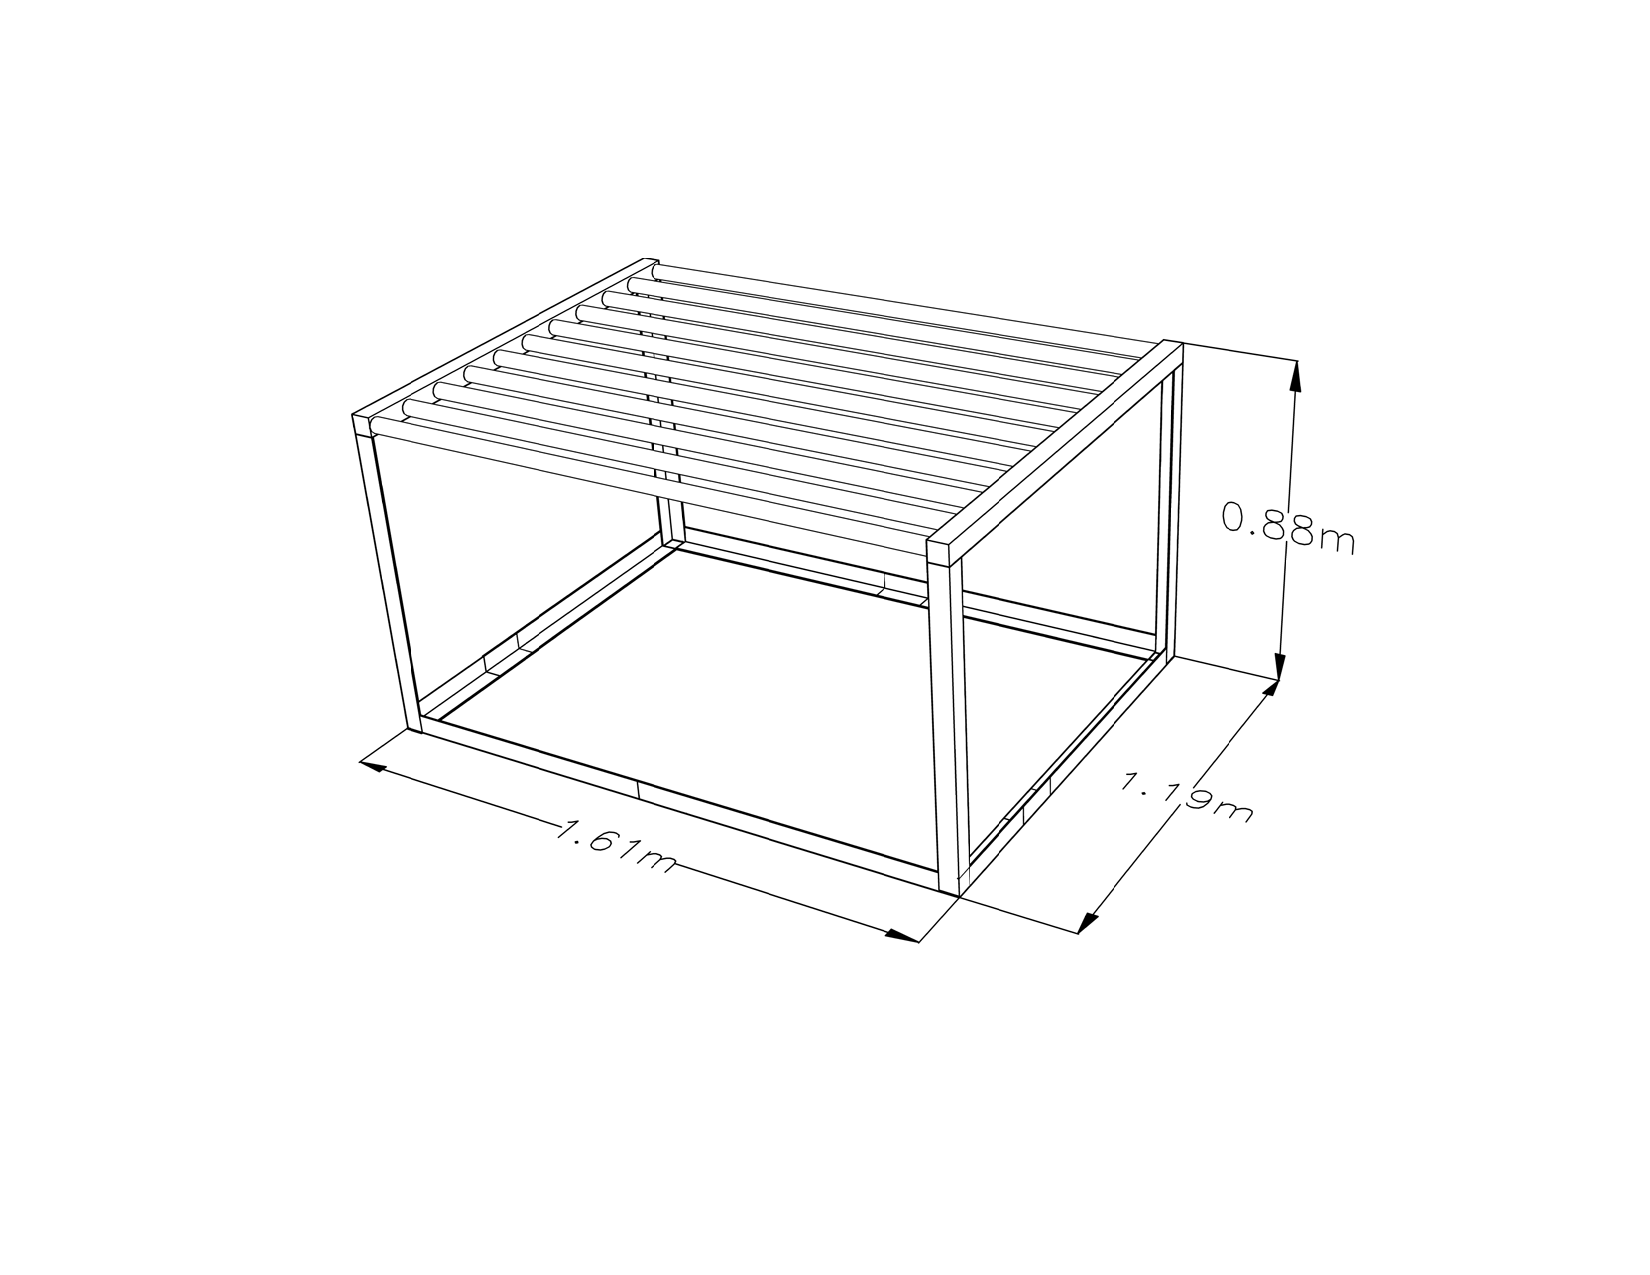
\includegraphics[width=.8\textwidth]{../Figures/Natural_Gas_Burner}
\caption {Isometric view of dimensioned natural gas burner.}
\label{fig:nat_gas_burn}
\end{figure}

The required mass flow of natural gas ($\dot{m}_{NG}$) needed to produce a desired fire size ($HRR_{NG}$) is
\begin{equation}
\dot{m}_{\mathrm{NG}} = HRR_{NG}/h_{c_{NG}}
\end{equation}
where $h_{c_{NG}}$ is the heat of combustion of natural gas. For complete combustion, the heat of combustion of natural gas is 50203 kJ/kg. Based on calculations included in \ref{app:gas_burn}, the required mass flow rate of natural gas for range of fire sizes is shown in Table~\ref{tab:ng_flow}. While the peak deliverable HRR is 8 MW, radiation from the fire to the surrounding environment at this magnitude is too significant for a 60 minute commissioning test. To test each train, a 4 MW fire will be used. To test that both trains can properly work together, an 8 MW fire will be used for a short duration, approximately 5 minutes. 

\begin{table}
\centering
\caption{Mass flow rate of natural gas for experimental range of HRRs}
\label{tab:ng_flow}
\begin{tabular}{cc}
\toprule[1.5pt]
Fire Size (MW) & Flow Rate (kg/s)  \\
\midrule
2  &  0.04 \\
4  &  0.08 \\
6  &  0.12 \\
8  &  0.16 \\
\bottomrule[1.25pt]
\end{tabular}\par
\end{table}

\section{Test 2}
\label{test2}
To challenge the acid scrubbing capability of the system, pinewood cribs loaded with polyvinyl chloride (PVC) are used. This package is designed to deliver a controlled source of hydrochloric acid (HCl) gas that is close to the design capacity of the emission control system. Four pinewood cribs measuring 0.56 m by 0.56 m by 0.38 m will be used (cf. Fig.~(\ref{fig:wood_crib})). Each crib consists of 10 layers composed of 0.56 m by 0.04 m by 0.04 m pinewood sticks spaced 0.02 m apart. Eight 0.45 kg PVC sticks are distributed throughout each crib (cf. Fig.~(\ref{fig:wood_crib})) which brings the total mass of each crib to be 34 kg. The moisture content of the cribs should be between 6-8 \% using a commercial moisture detector. This fuel package is based on the wood crib tests from the 2001 commissioning tests.

\begin{figure}
\centering
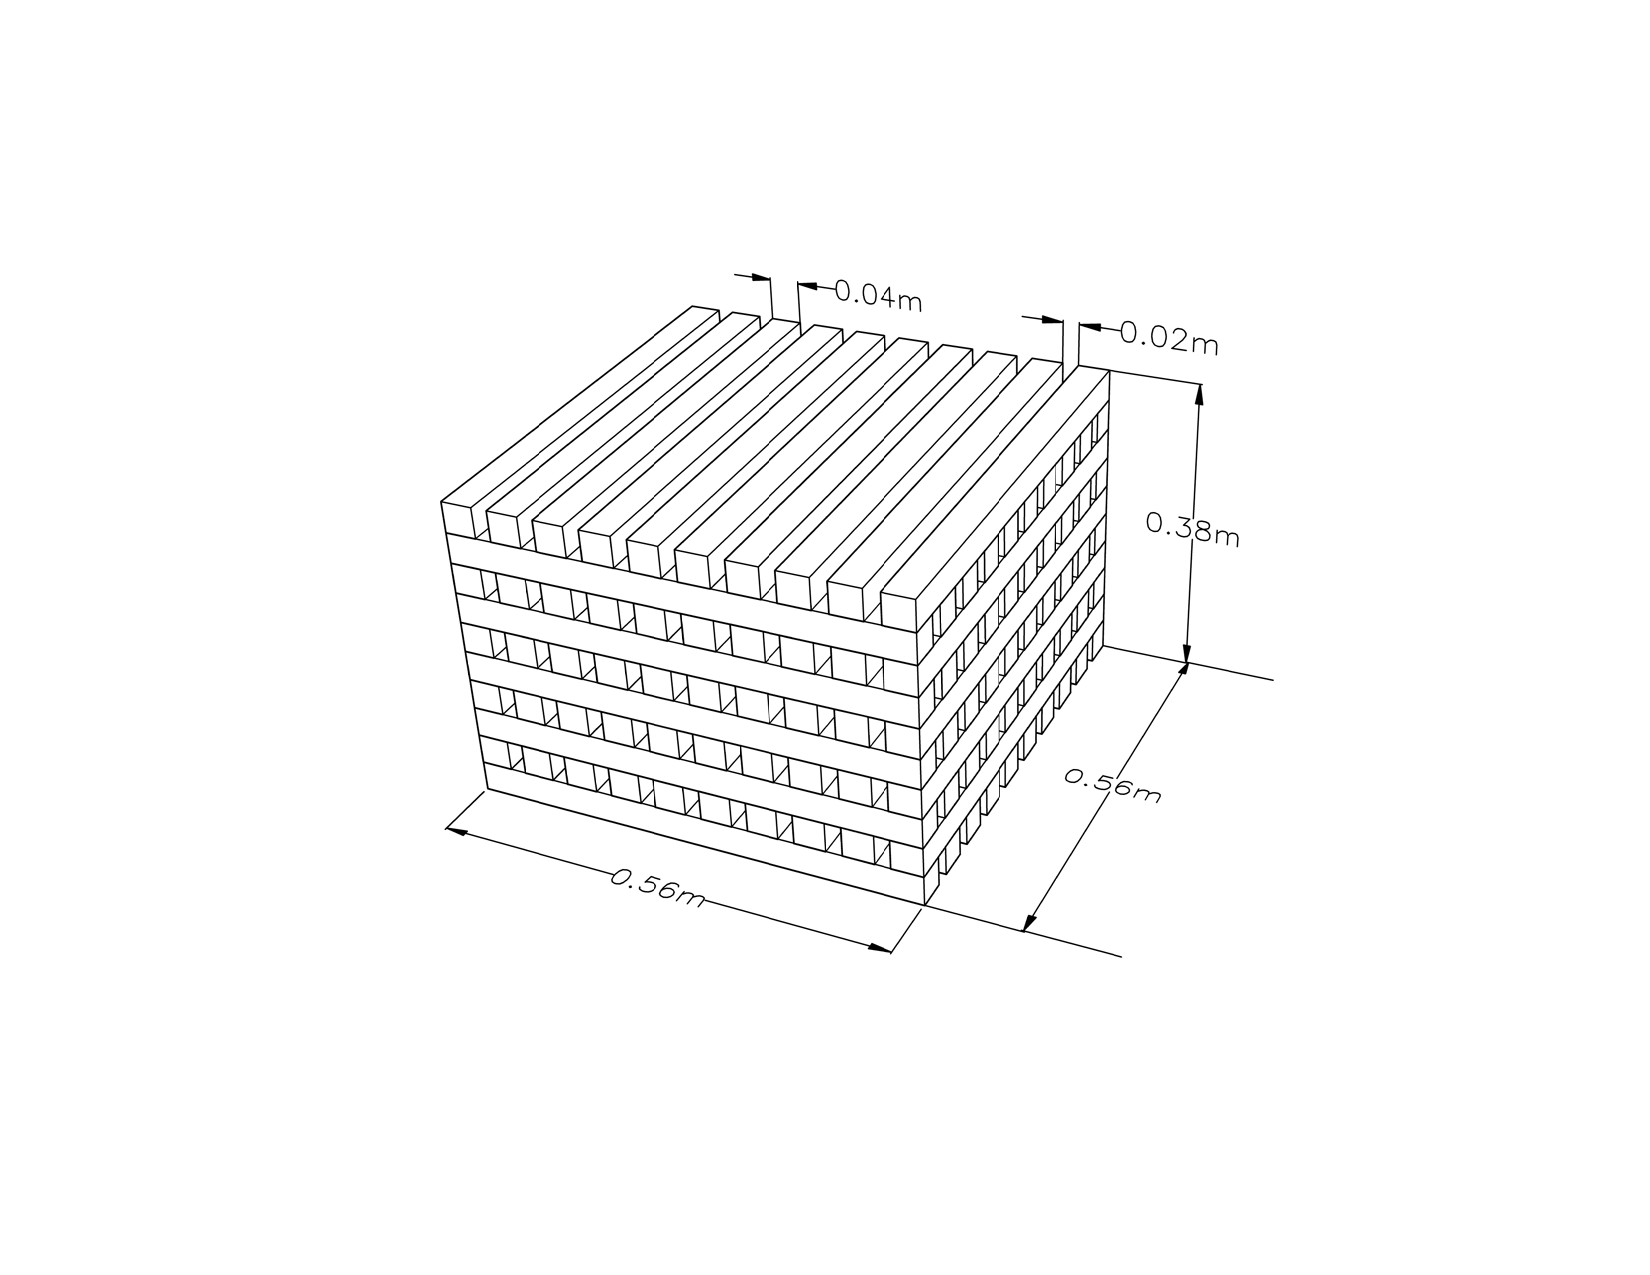
\includegraphics[width=.75\textwidth]{../Figures/Wood_Cribs}
\caption {Isometric view of dimensioned single wood crib.}
\label{fig:wood_crib}
\end{figure}

To determine the HCL yield of PVC, we need to determine a balanced chemical reaction. First, is to assume that the test PVC can be represented by the chemical formula, $\C_2\H_3\Cl$ and that all of the Cl in PVC goes to HCl. Then, based on work by Tewarson \cite{SFPE:Tewarson}, yields for soot and CO are found ($y_{\mathrm{C}}$= 0.172, $y_{\mathrm{CO}}$= 0.063) and a balanced chemical reaction is created:

\begin{multline}
\C_2\H_3\Cl \,+\, 7.29(0.21 \O_2 \,+\, 0.79 \N_2) \\
\rightarrow 9.76(0.102\HCl \,+\, 0.103\H_2\O \,+\, 0.014 \C\O \,+\, 0.098 \C\O_2 \,+\, 0.092 \C \,+\, 0.59 \N_2)
\label{eq:hcl_reac}
\end{multline}
Based on Eq.~(\ref{eq:hcl_reac}), there is a 58 \% mass basis theoretical yield of HCl (\ref{app:crib}).  Experimental data based on burning PVC over a wide range of test conditions and using a wide range of measurement techniques puts the HCl yield between 10 and 56 \% \cite{Leeds:PVC}. Using data for a similarly scaled and ventilated test, the estimated HCl yield is 32 \% \cite{Persson1998}. Since each crib contains 3.63 kg of PVC and the test calls for 4 cribs, the expected yield of HCl at the source fire is 4.65 kg (10.2 lb). Based on an estimated 60-70 \% loss of HCl to gas phase conversion and reaction through the duct work, the estimated mass of HCL upstream of the scrubber is 1.4-1.9 kg (3-4 lb).

The 4 cribs will be setup in two tiers. The first tier will be three cribs arranged in a triangle. The second tier will use the forth crib centered over the void created by the triangle. Each of the lower tier cribs will be raised 0.08 m off the ground to allow for a pan of heptane to slide underneath. The test configuration is shown in Fig.~(\ref{fig:test_crib}).The cribs are ignited using 500 mL of heptane poured into a round steel pan. The heptane represents about 1.5 \% of the initial mass of the crib, and burns out after about 2.5 to 3 minutes. The forth crib will ignite as a result of flame spread from the other three cribs.

\begin{figure}
\centering
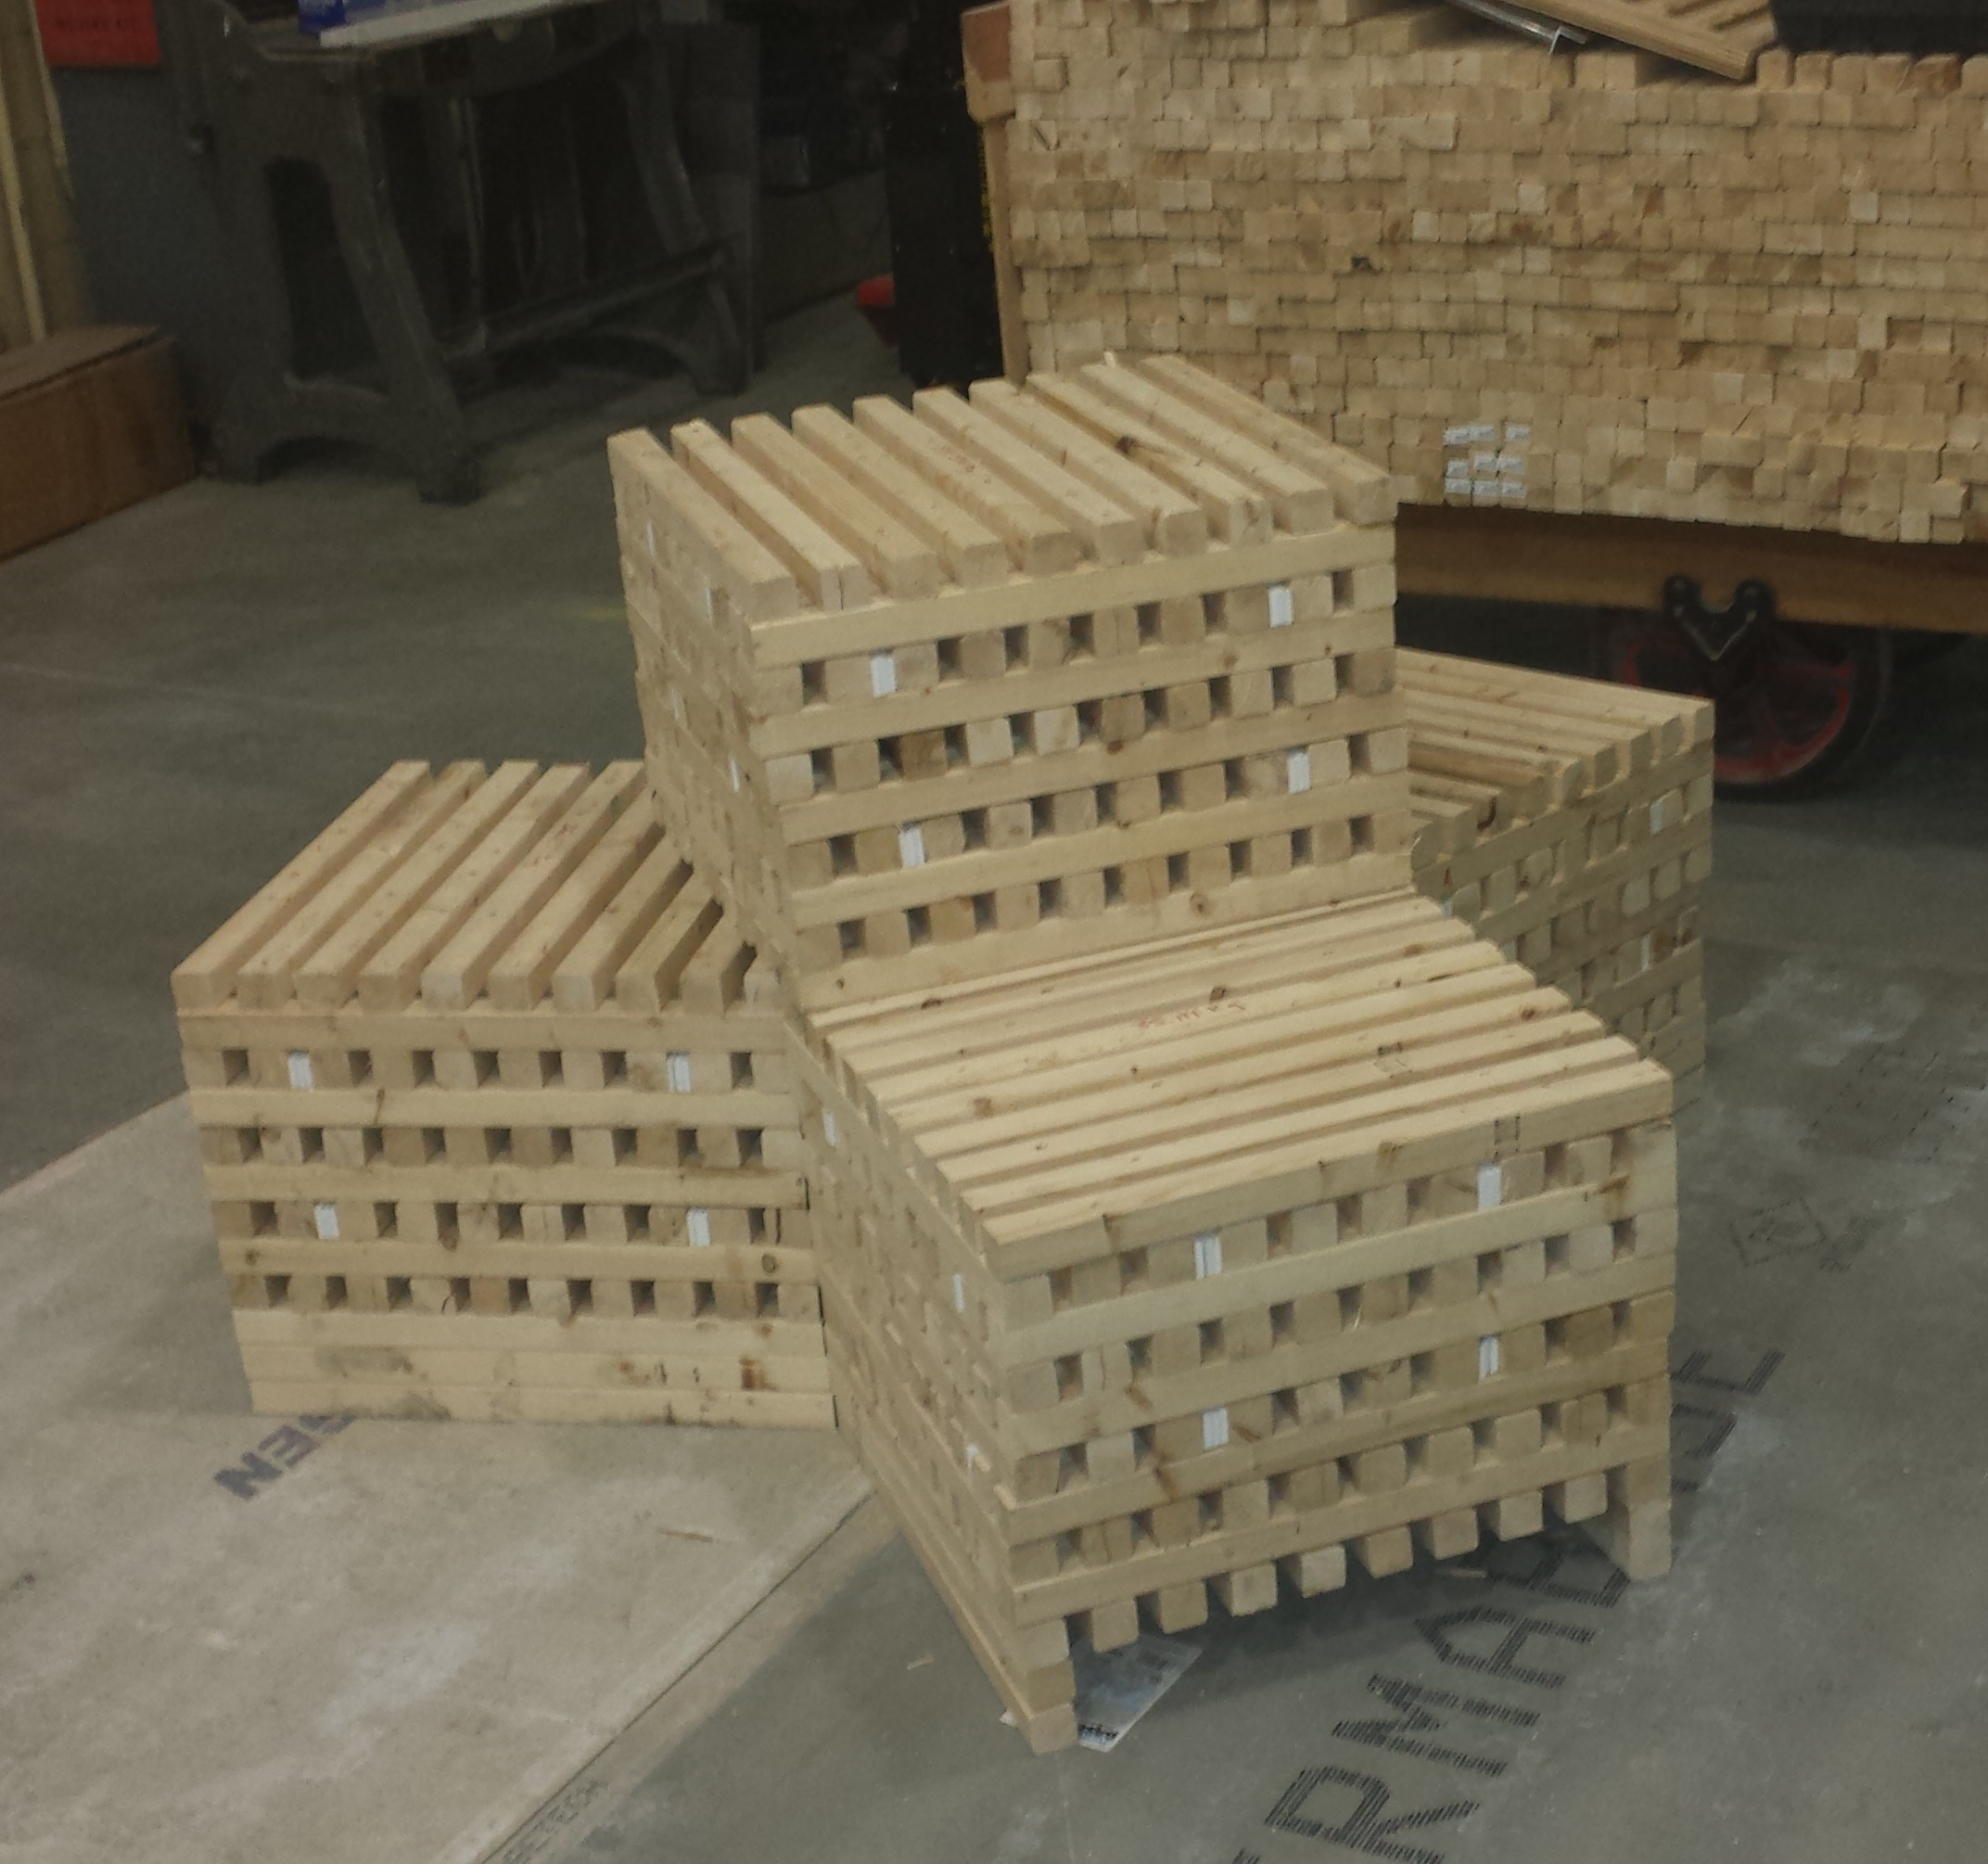
\includegraphics[width=.7\textwidth]{../Figures/cribs}
\caption {Test configuration of 4 wood cribs with PVC inserts.}
\label{fig:test_crib}
\end{figure}

The burning rate of wood cribs is found from experiments performed by Madrzykowski and Stroup \cite{Madrzykowski1998} and Bryner and Mulholland \cite{Bryner1991}. The steady burning rate averaged over the peak 50 \% of burning is 0.03 kg/s. If an entire 34 kg crib burned at this rate, the burn would last approximately 19 minutes. If we estimate that 50 \% of the mass burns at 0.03 kg/s and the remaining 50 \% burns at $1/3$ the burning rate, 0.01 kg/s, then a crib burn would take approximately 40 minutes. The bottom three cribs in Fig.~(\ref{fig:test_crib}) are all ignited at nominally the same time. Therefore we can assume that all three will burn for about 40 minutes. If we assume an ignition delay of 5 minutes, a conservative estimate for total burn time is 45 minutes. This falls into the range of experimental burn durations from \cite{Bryner1991} of 40 to 65 minutes.

Wood cribs typically have peak HRR that range between 300 kW to 500 kW \cite{Madrzykowski1998,Bryner1991}. Depending on the time to peak HRR of first tier cribs relative to the second tier crib, the estimated peak HRR for these experiments is between 1.5 MW to 2 MW. 

\section{Test 3}
\label{test3}
The third commissioning test is designed to test the system's capability to handle particulates, specifically soot. Standard Group A commodity boxes will be used as the fuel source. Each box, is a cube 0.53 m on a side and is filled with a plastic commodity. The plastic commodity inside the box consists of rigid crystalline polystyrene cups (empty, 0.47 L (16 fl oz) size) packaged in compartmented, single-wall, corrugated cardboard box. The cups are arranged open end down in five layers, 25 per layer for a total of 125 per box (cf. Fig.~(\ref{fig:open_box})).

\begin{figure}
\centering
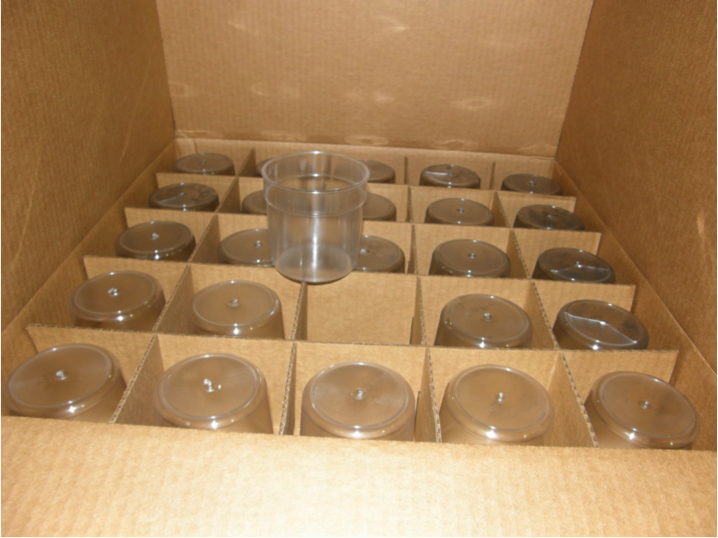
\includegraphics[width=.7\textwidth]{../Figures/open_box}
\caption {Open commodity box showing top row of polystyrene cups.}
\label{fig:open_box}
\end{figure}

The mass of a polystyrene cup is 36 g. Using the 125 cup per box specification, there is 4.5 kg of polystyrene in each box. Using a soot yield of 0.16 kg soot/kg polystyrene from Tewarson \cite{SFPE:Tewarson}, then each box should produce approximately 0.72 kg of soot. Based on experimental work for the NYU-Poly ALIVE program \cite{Madrzykowski2013}, two columns of boxes with three rows of boxes in each column will burn between 20 to 25 minutes with a peak HRR of $\approx$ 2.5 MW. The six Group A commodity boxes should produce a total soot yield of 4-4.5 kg ($\approx$ 9 lb). Following the same analysis as the soot prediction and using an unburned hydrocarbon yield of 0.014 kg HC/kg polystyrene \cite{SFPE:Tewarson}, the boxes should produce approximately 0.4 kg (0.89 lb) of unburned hydrocarbons. This results in 0.96 to 1.2 kg of unburned hydrocarbons per hour (2.1 $-$ 2.6 lb/hr).

In these tests, the columns of boxes are spaced 0.15 m apart (cf. Fig.~(\ref{fig:dim_box})). It is important to note that both orientation and spacing of these boxes can have a significant impact on the burning characteristics \cite{Madrzykowski2013}.

\begin{figure}
\centering
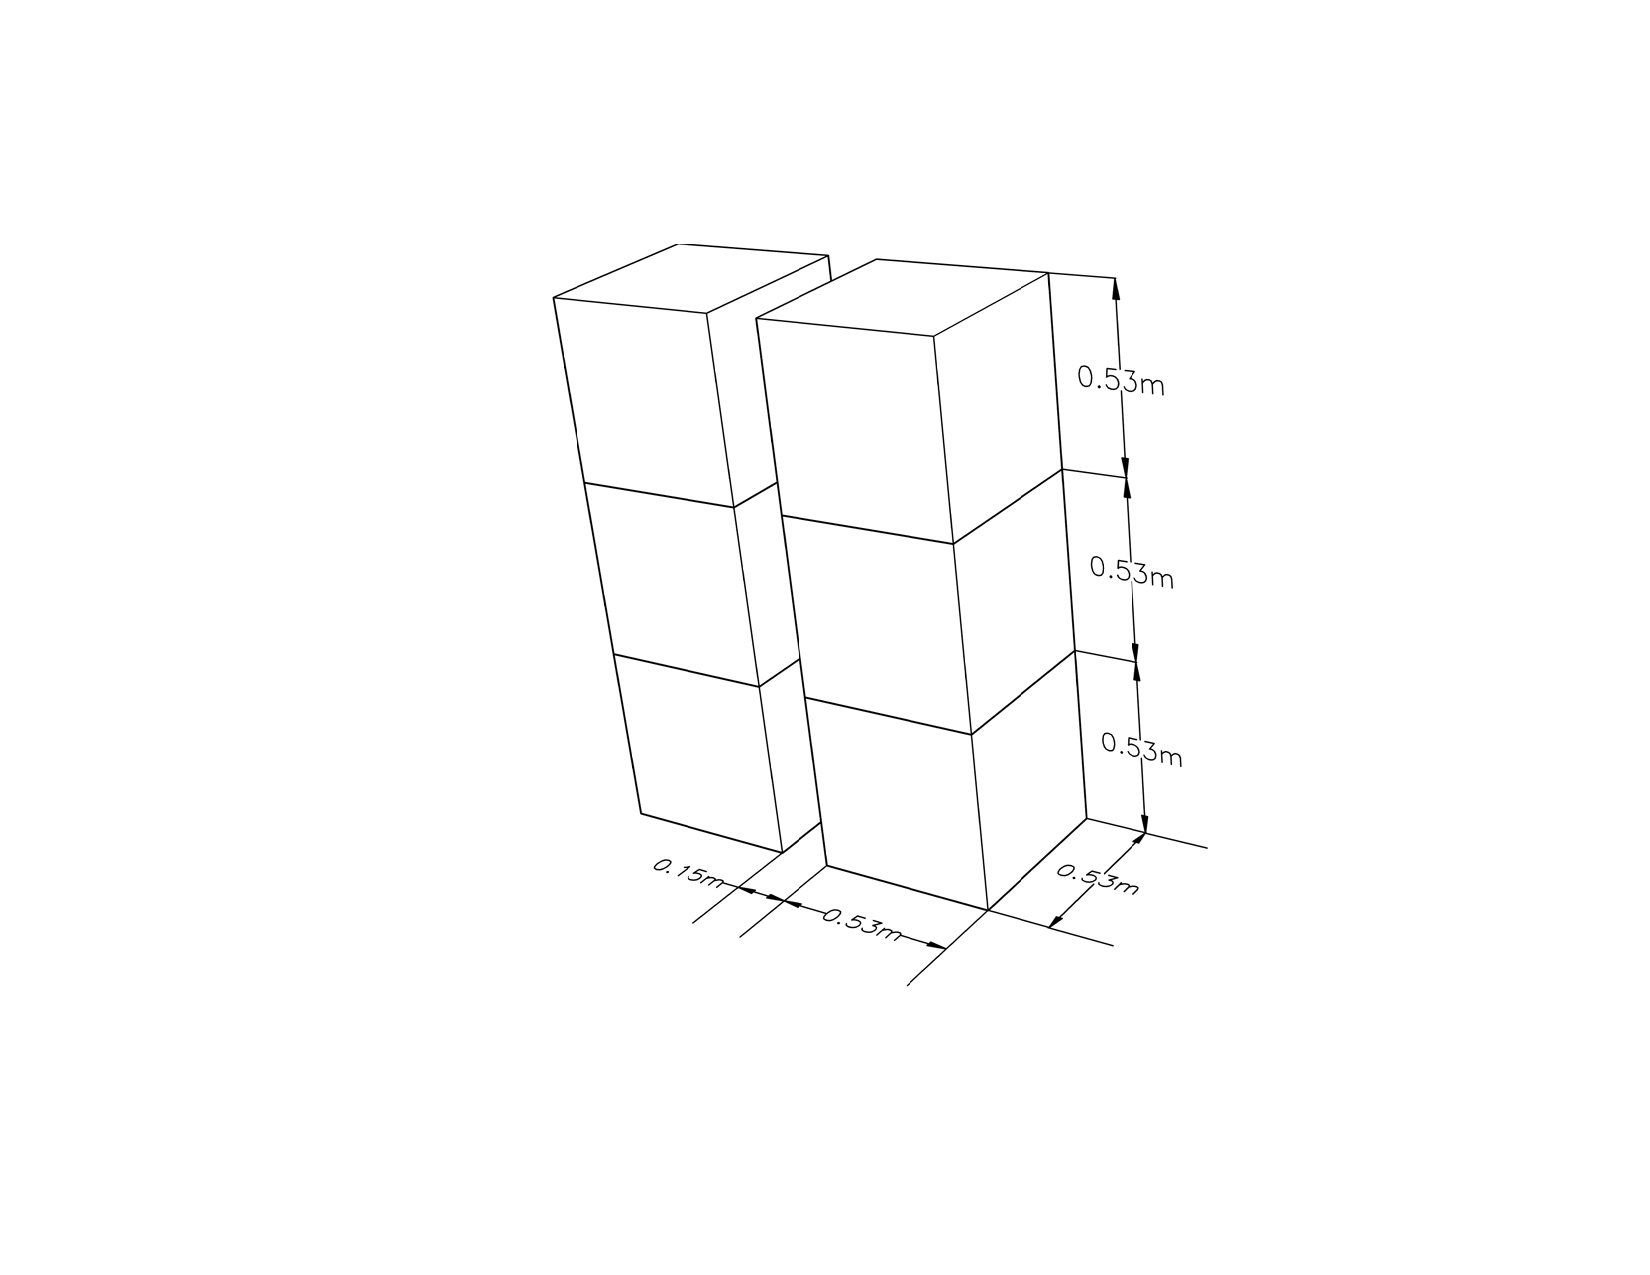
\includegraphics[width=.7\textwidth]{../Figures/dim_box_array}
\caption {Dimensioned array of commodity boxes in test configuration.}
\label{fig:dim_box}
\end{figure}

The two columns of boxes will be ignited using shredded paper placed in the gap between the two columns of boxes. The paper will be ignited by a 1.83 m (6 ft) propane wand. As the cardboard burns away, the columns will lose structural integrity and the fire will transition into a polystyrene pool fire. The ignition point is set at the center line so that as the columns begin to collapse, they will collapse toward the center as that cardboard burned away first. The experiment will take place on top of sheets of cement board (such as USG Durock). This is done to contain the polystyrene melt in the later portion of the fire test. Fig.~(\ref{fig:comm_burn}) shows two columns of Group A commodity shortly after ignition and when the boxes are fully involved.

\begin{figure}[!ht]
\begin{tabular*}{\textwidth}{l@{\extracolsep{\fill}}r}
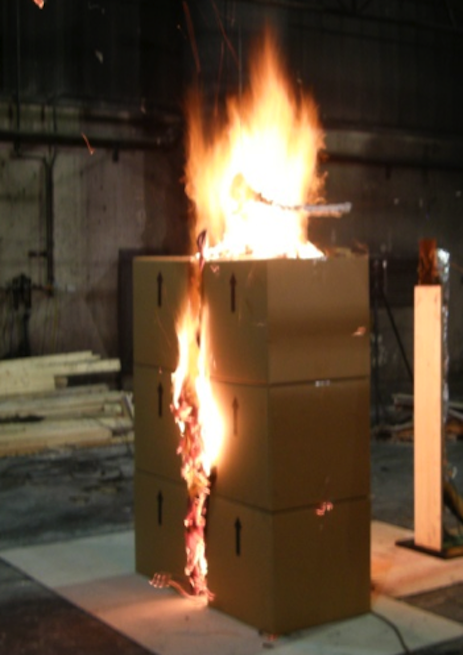
\includegraphics[width=0.45\textwidth]{../Figures/comm_ignite} &
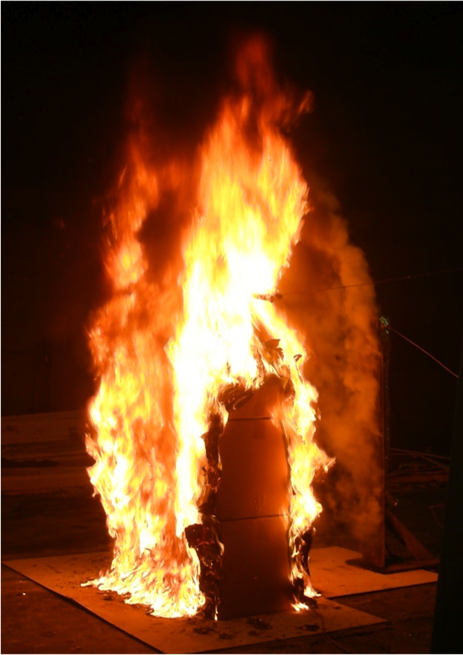
\includegraphics[width=0.45\textwidth]{../Figures/comm_burn} \\
\end{tabular*}
\caption{Two stacks of 3 boxes of group A commodities just after ignition (left) and fully involved (right). The boxes are lit with shredded paper and an electric match.  Peak heat release is $\approx$ 2.5 MW.}
\label{fig:comm_burn}
\end{figure}


\chapter{Safety}
\label{safety}
\section{Lab Safety Controls}
\label{controls}
At least two members of the NIST Fire Department will be present to perform a pre-test inspection and emergency fire suppression. A safety briefing will be connected prior to each test. All test participants and observers must attend the safety briefing. The occupancy in the lab during the commissioning fires will be determined by the AHJ. Test specific emergency procedures must be reviewed at each safety briefing.

\section{Potential Lab Hazards}
\label{lab_hazards}
For the ECS commissioning tests at the NFRL, the building will be transitioning from a construction site to an active laboratory. This combination space presents safety hazards to occupants. A partial lists of hazards to consider follows:
\begin{itemize}
\item {\bf Electrical Hazards}
%Minimum personal protective equipment (PPE) is safety glasses with side shields and steel toed safety shoes. Equipment, power cords and general housekeeping are inspected on a regular basis by Workspace Manager. Users of equipment in this workspace must have completed electrical safety training. All wall outlets are appropriately marked with voltage and breaker box number/breaker number.
\item {\bf Toxic/Corrosive Chemicals}
%All workers in this lab must complete MSDS training. CO detectors are installed near the CO cylinder and throughout work areas.  All NFRL staff members and guest workers are equipped with personal CO monitors that alarm at 10 ppm. Post fire test specimens (such as mattresses, furniture and demolished burn room structures that must be removed from building 205 are doused with water and stored in the rented construction dumpster). A thermal imaging camera will be used to insure samples have been fully extinguished before placing in this dumpster. Appropriate protective clothing and breathing apparatus will be determined according to the hazards associated with disposal of post-project debris.
\item {\bf Flammable/Reactive Materials}
%Minimum PPE is safety glasses with side shields and steel toed safety shoes. Two permanent flammable gas alarms are located above the natural gas fuel delivery line in the ceiling area. Protective barrier posts are installed at the base of the natural gas line to prevent vehicle collision. The gas line is equipped with three quarter turn shutoff valves and an automatic safety shutoff valve (secured with a key to prevent unintended use). A quarter turn valve located on the south side of building 205 can be used to shut off the gas supply to the entire building.  The natural gas flow rate and pressure are monitored when the burner is in use.
\item {\bf High Pressure Fluid Flow}
%Minimum PPE is safety glasses with side shields and steel toed safety shoes. Fire hose stream operators must complete MFRI fire suppression training and NFRL WSM led training.  Fire hose lines are routinely inspected and checked for leaks and taken out of service when leaks are found. Standpipe valves are closed and secured when not in use. A minimum of two qualified operators are required to handle a hose stream suppression line. 
\item {\bf Moving Heavy Objects}
%A forklift, hand truck, pallet jack, hoist crane and/or skid loader will be utilized to lift and move heavy objects that cannot be moved by hand. All operators will be adequately trained to use these devices. Training records must be documented in an approved project FLHR document before the start of any activity with this equipment.
\end{itemize}

\chapter{Experimental Test Procedures}
\label{test_procedure}
\section{Test 1 Procedure}
\label{procedure1}

\begin{enumerate}
  \item Perform leak check on all burner gas line connections and valves.
  \item Perform visual inspection to ensure spark ignitors are functioning correctly.
  \item Use a small flame to prove flame detector fuel shutoff safety system is working and will stop fuel flow if no flame is visible by shutting the Maxon safety shutoff valve.
  \item Start data collection system.
  \item Energize spark ignition system.
  \item Open pilot tube solenoid valve
  \item Slowly open manual metering valve and set fire to 100 kW.
  \item Open burner solenoid valves for banks 1 and 2 and set the fire to 500 kW.
  \item Open burner solenoid valves for banks 3 and 4 and set the fire to 2000 kW.
  \item After 15 min, slowly open the manual control valve to 4000 kW.
  \item After 15 min, slowly close the control valve and burner bank tubes and set the fire to 100 kW.
  \item Shut off the Maxon safety valve and then shut off the pilot tube after the fire is out.
  \item Close the manual shutoff valve. Wait 20 min before handling the burner.
\end{enumerate}

\section{Test 2 Procedure}
\label{procedure2}
\begin{enumerate}
  \item All flammable liquid stored are in outdoor containment building with a fuel spill containment floor. 
  \item A secondary containment device (graduate cylinder) will be used when transferring fuels and conducting fire tests.
  \item Position wood cribs on cement board.
  \item Fill 3 ignition pans with 500 mL heptane.
  \item Slide each pan of heptane under one of three wood cribs. 
  \item Ignite fuel pans with a 1.83 m (6 ft) propane wand ignitor.
  \item Verify all post fire materials are sufficiently cool to prevent smoldering or off gassing.
  \item Workers are required to use PPE when performing post-fire cleanup.

\end{enumerate}

\section{Test 3 Procedure}
\label{procedure3}
\begin{enumerate}
  \item Position commodity boxes on cement board.
  \item Position shredded paper ignition source in 0.15 m gap between stacked boxes.
  \item Ignite shredded paper with 1.83 (6 ft) propane wand ignitor.
  \item Verify all post fire materials are sufficiently cool to prevent smoldering or off gassing.
  \item Workers are required to use PPE when performing post-fire cleanup.
\end{enumerate}



\chapter{Results}
Seven tests were conducted to commission the NFRL ECS:
\begin{enumerate}
\item 4 MW natural gas burn, exhaust train 3
\item 4 MW natural gas burn, exhaust train 4
\item 8 MW natural gas burn, exhaust trains 3 and 4
\item Wood crib burn, ECS train 3
\item Commodity burn, ECS train 3
\item Wood crib burn, ECS train 4
\item Commodity burn, ECS train 4
\end{enumerate}
Emission measurements were not made for tests 1, 2, and 3 since they were natural gas tests. Measurements were made during tests 4, 5, 6 and 7. The measurements were taken at the exhaust stack; the farthest downstream sensor port in the ECS.  Data was recorded throughout the duration of the experiments and then time averaged. Table~\ref{tab:hcl_data} shows the results including the mean mass flow rate of HCl for tests 4 and 6 as well as from a similar test conducted in 2001.

\begin{table}[!ht]
\centering
\caption{Exhaust measurements for wood crib experiments}
\label{tab:hcl_data}
\begin{tabular}{cccc}
\toprule[1.25pt]
Measurement Quantity & Test 4 & Test 6 & 2001 Test  \\
\midrule
Metered Volume (dcf)           &  47.39  &  59.22  &  36.52  \\
Total Test Time (min)          &  56.1   &  68.3   &  60     \\
Gas Temperature ($^{\circ}$F)  &  285    &  296    &  268    \\
Oxygen (\%)                    &  19.16  &  19.56  &  19.7   \\
Carbon Dioxide (\%)            &  0.81   &  1.00   &  1.1    \\
Velocity (ft/s)                &  54.37  &  54.36  &  45.09  \\
HCl Concentration (ppmdv)      &  8.60   &  10.55  &  2.98   \\
Mass Rate (lb/hr)              &  2.96   &  3.57   &  0.86   \\
\bottomrule[1.25pt]
\end{tabular}\par
\end{table}

Table~\ref{tab:part_data} shows the results including particulate emissions for tests 5 and 7.

\begin{table}[!ht]
\centering
\caption{Exhaust measurements for commodity experiments}
\label{tab:part_data}
\begin{tabular}{ccc}
\toprule[1.25pt]
Measurement Quantity & Test 5 & Test 7  \\
\midrule
Metered Volume (dcf)                &  40.97  &  38.28  \\
Total Test Time (min)               &  48.1   &  43     \\
Gas Temperature ($^{\circ}$F)       &  288    &  300    \\
Oxygen (\%)                         &  18.92  &  19.36  \\
Carbon Dioxide (\%)                 &  0.99   &  0.91   \\
Velocity (ft/s)                     &  53.75  &  55.18  \\
Particulate Concentration (g/dscf)  &  $< 4.67\text{\sc{e}-}5$   &  $< 5.08 \text{\sc{e}-}5$  \\
Mass Rate (lb/hr)                   &  $<$ 0.37   &  $<$ 0.40   \\
\bottomrule[1.25pt]
\end{tabular}
\end{table}


\chapter{Summary}

\chapter{Acknowledgments}

\bibliography{../../../Bibliography/FDS_refs,../../../Bibliography/FDS_general,ECS}

\newpage

\appendix
\chapter{Schematics of the National Fire Research Lab}
\label{app:nfrl_images}
\begin{figure}[!ht]
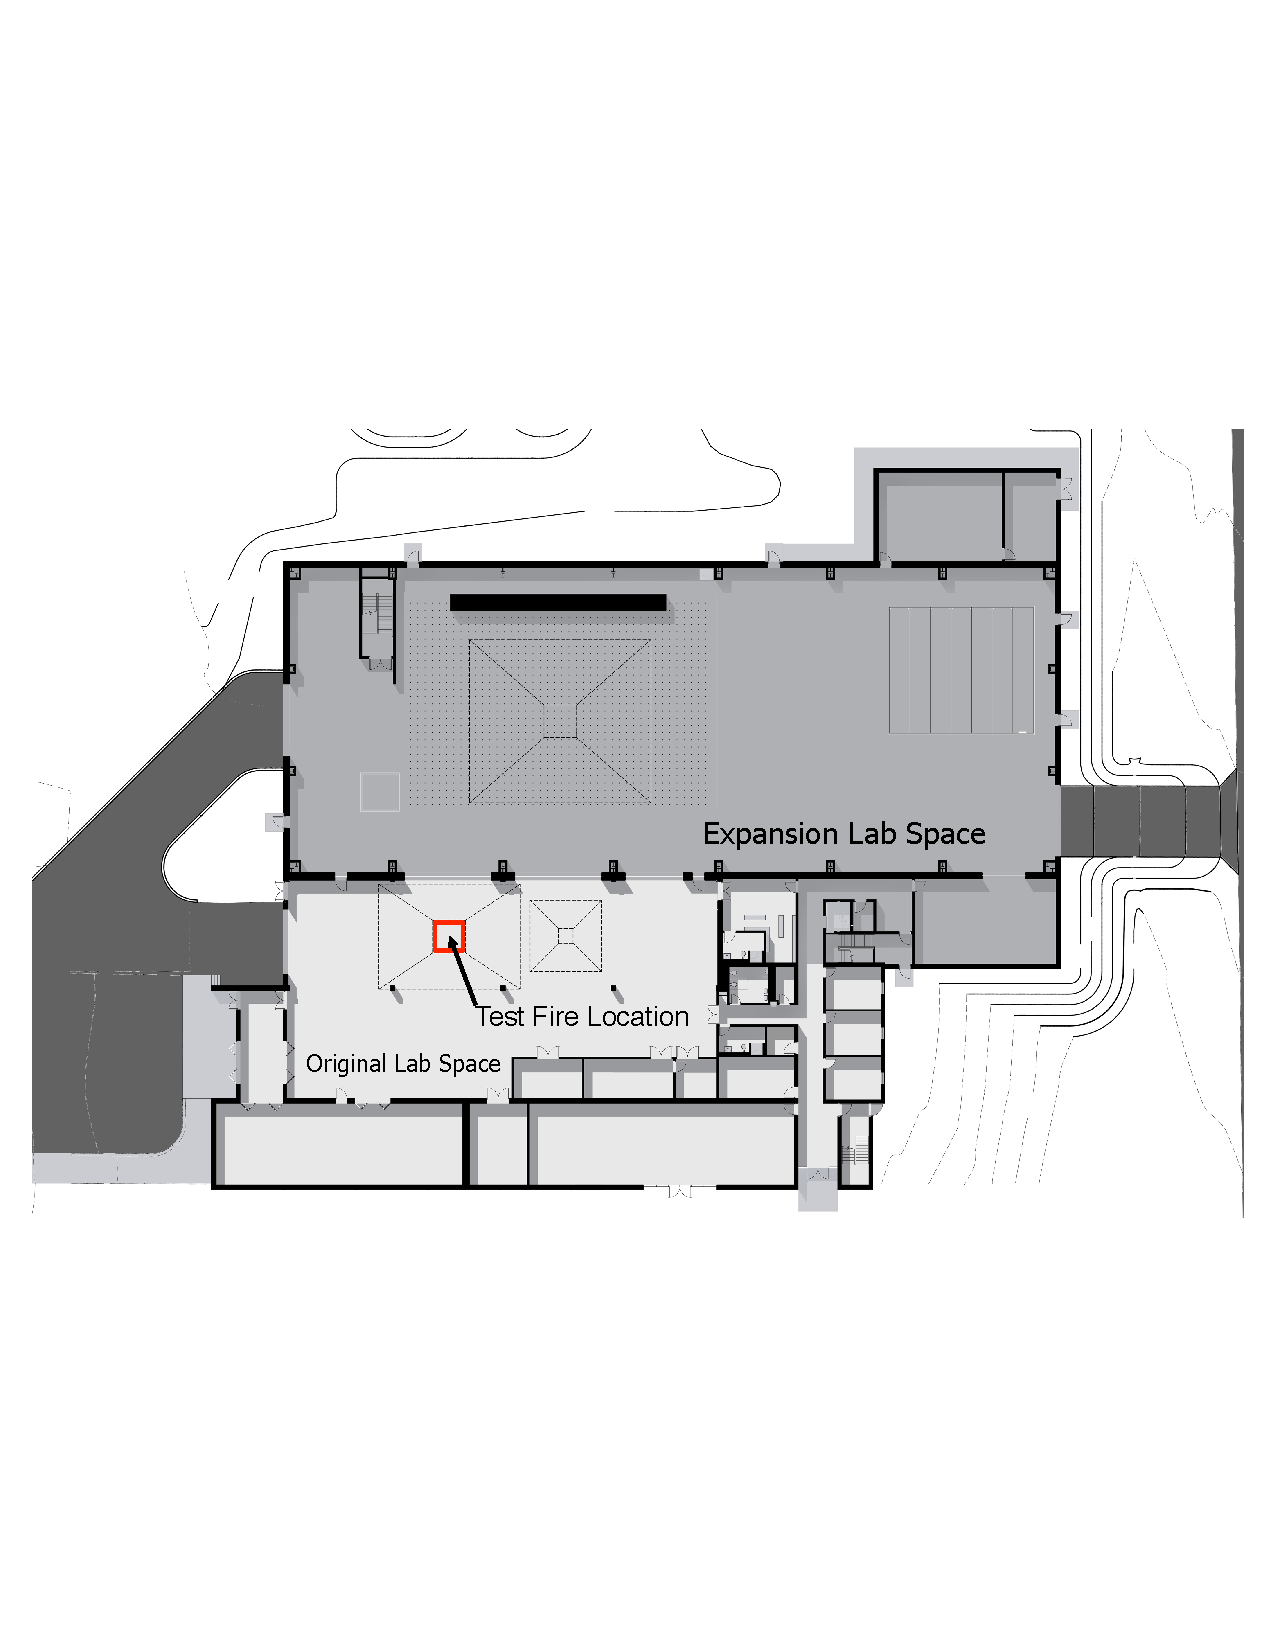
\includegraphics[width=\textwidth]{../Figures/plan_view2}
\caption {Plan view of the NFRL indicating location of ECS test fires.}
\label{fig:NFRL_plan}
\end{figure}

\begin{figure}[!ht]
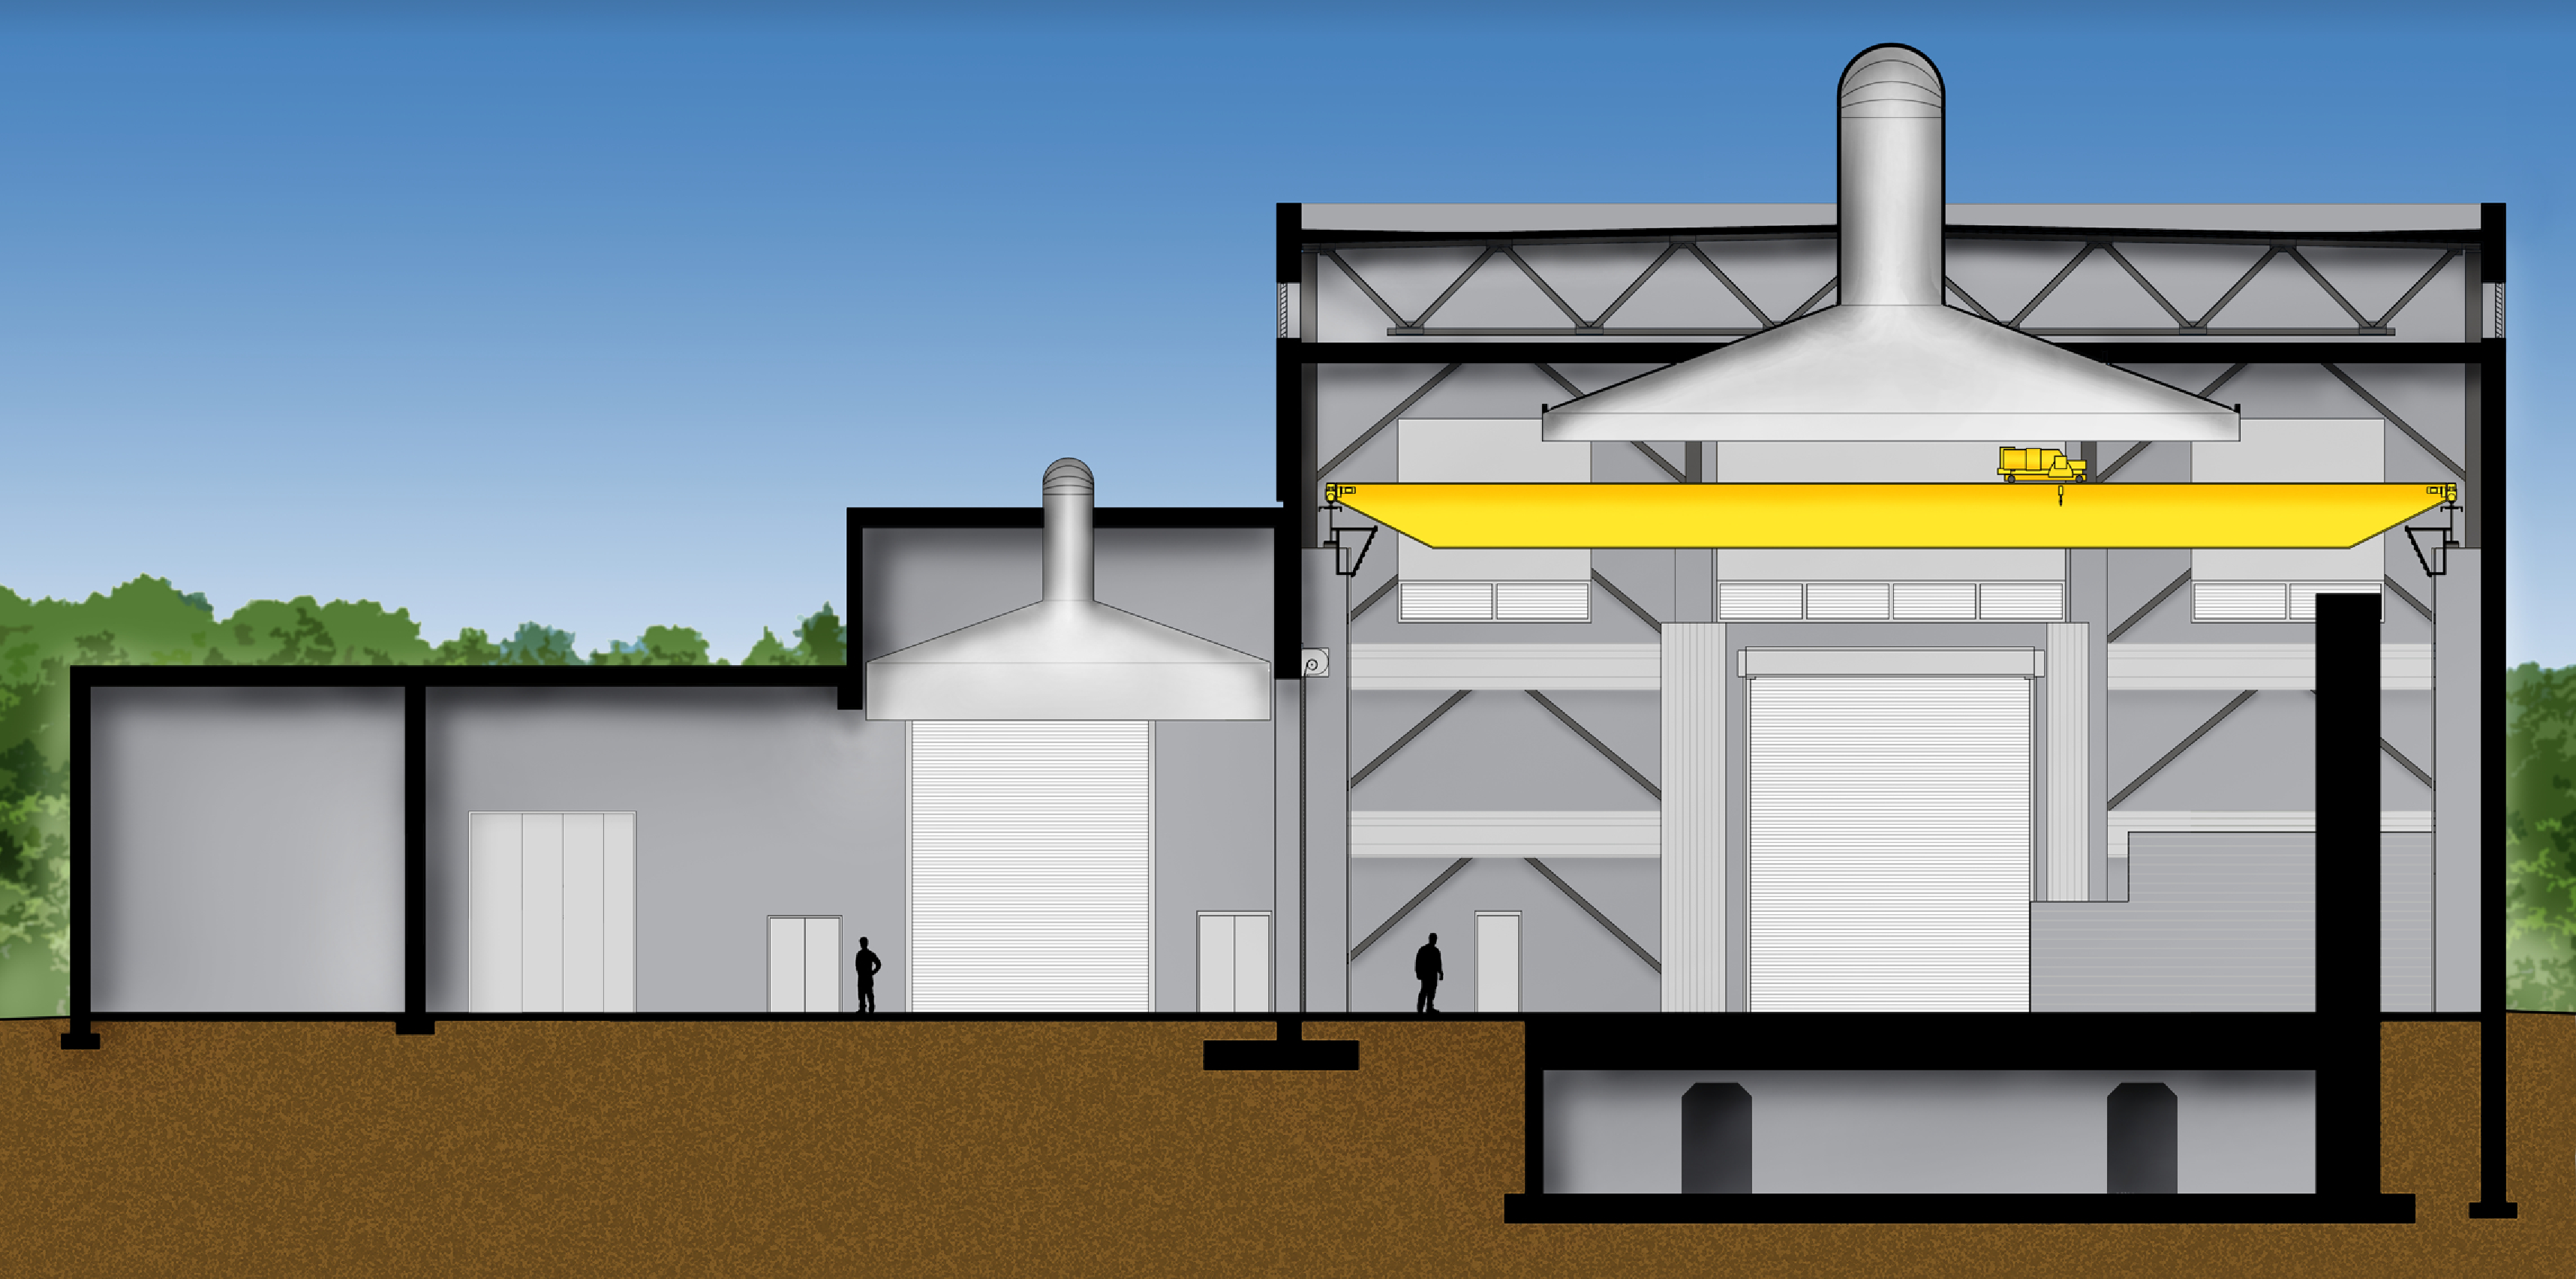
\includegraphics[width=\textwidth]{../Figures/section_2}
\caption {Rendering of the NFRL showing the original lab space (left) and the new lab space (right).}
\label{fig:NFRL_render}
\end{figure}
\end{document}
